\documentclass[slidestop,compress,mathserif,10pt]{beamer}

\mode<article> % 仅应用于article版本
{
  \usepackage{beamerbasearticle}
%  \usepackage{fullpage}
  \usepackage{hyperref}
}

%% 下面的包控制beamer的风格,可以根据自己的爱好修改
\usepackage{beamerthemesplit}   % 使用split风格
\usepackage{beamerthemeshadow}  % 使用shadow风格
%\usepackage[width=2cm,dark,tab]{beamerthemesidebar}
%\usepackage{beamerthemetree}
%\usetheme{Montpellier}
%\usecolortheme{lily}


%% 这些包是可能会用到的,不必修改
\usepackage{amsmath,amssymb}
\usepackage{graphicx}
%\usepackage{color}
%\usepackage{pgf,pgfarrows,pgfnodes,pgfautomata,pgfheaps}
%\usepackage{multimedia}

%\documentclass{beamer}
%\usepackage{beamerthemeshadow}
\usepackage{beamerthemesplit}
%\usetheme{shadow}
\usepackage{graphicx}
\usecolortheme{lily}
%\usepackage{amsmass}
\usepackage{amssymb,amsfonts,url}
\graphicspath{{Problems/}}

%\usepackage{CJK}
%\usepackage{pinyin}

%    \begin{figure}
%        \centering
%        \includegraphics[width=0.8\textwidth]{newGeneRep.eps}
%    \end{figure}

% \begin{figure}%
%   \begin{center}%
%     \begin{minipage}{0.70\textwidth}%
%      \includegraphics[width=1.0\textwidth]{comp25000.eps}%
%     \end{minipage}%
%     \begin{minipage}{0.30\textwidth}
%      \includegraphics[width=1.0\textwidth]{comparelabel.eps}%
%     \end{minipage}%
%   \end{center}
% \end{figure}

% \begin{table}
%   {\begin{tabular}{l|rrr}\hline
%       & \multicolumn{3}{c}{Actual number of DCJ operations}\\
%       \# genes &\# genes $\times 1$&\# genes $\times 2$&\# genes  $\times 3$ \\
% \hline
%      (a)~25,000 & 0.5\% ~~&  0.9\% ~~& 1.7\%~~\\
%       (b)~10,000 & 0.8\%~~ &  1.4\% ~~& 2.7\%~~\\
%      (c)~ 1,000 & 2.7\%~~ & 4.7\%~~ & 14.7\%~~\\ \hline
%     \end{tabular}} {}%
% \end{table}

% \begin{eqnarray}
% T(n) &=&  \sum\nolimits_{i=1}^n C_i \\
%      &=&  \# PUSH + \#POP \\
%      &<& 2\times \#PUSH \\
%      &<& 2n \\
% \end{eqnarray}

% \[ 
% \begin{matrix}
% \begin{pmatrix}
% C_{11} & C_{12} \\ 
% C_{21} & C_{22} 
% \end{pmatrix}
% =
% \begin{pmatrix}
% A_{11} & A_{12} \\ 
% A_{21} & A_{22}  
% \end{pmatrix}
% 
% \begin{pmatrix}
% B_{11} & B_{12} \\ 
% B_{21} & B_{22}  
%  
% \end{pmatrix}
%     
%    \end{matrix}
% \]
% 
% 
% \begin{eqnarray}
%  C_{11} &=& (A_{11}\times B_{11}) + (A_{12} \times B_{21}) \\
% C_{12} &=& (A_{11}\times B_{12}) + (A_{12} \times B_{22}) \\
% C_{21} &=& (A_{21}\times B_{11}) + (A_{22} \times B_{21}) \\
% C_{22} &=& (A_{21}\times B_{12}) + (A_{22} \times B_{22}) 
% \end{eqnarray}
% \begin{figure}%
%      \begin{minipage}{0.32\textwidth}%
%       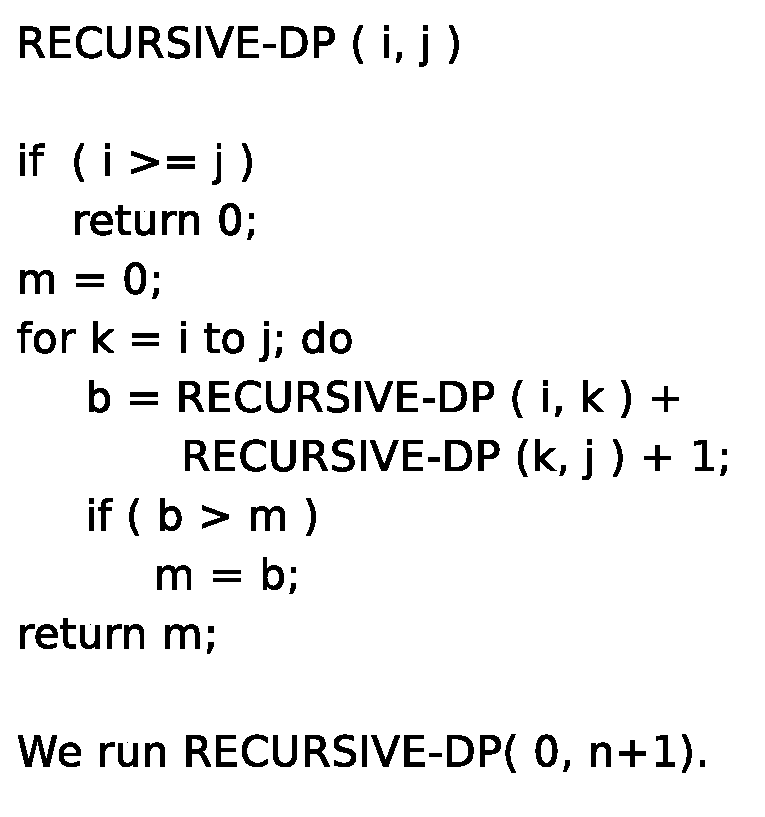
\includegraphics[width=1.0\textwidth]{L7-intervalschedulingdpalgo.eps}%
%      \end{minipage}%
%  \quad
%      \begin{minipage}{0.30\textwidth}
%       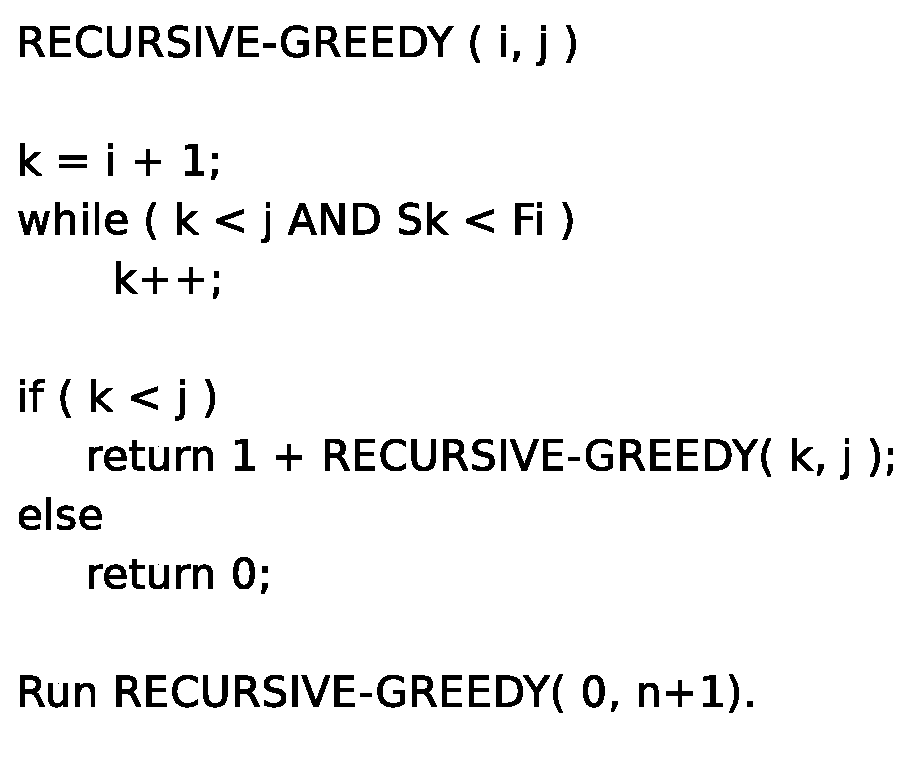
\includegraphics[width=1.0\textwidth]{L7-intervalschedulinggreedyalgo.eps}%
%      \end{minipage}%
%  \quad
%       \begin{minipage}{0.25\textwidth}
%       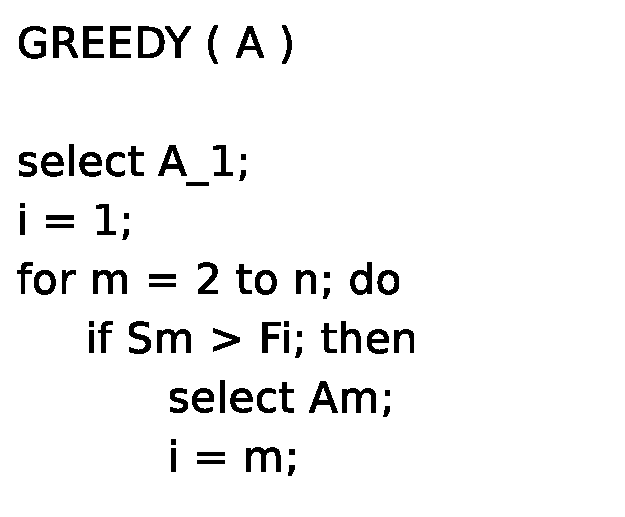
\includegraphics[width=1.0\textwidth]{L7-intervalschedulinggreedyalgo2.eps}%
%      \end{minipage}%
% 
%  \end{figure}

\title{CS612  Algorithm Design and Analysis }
\subtitle{ Lecture 19. {\sc Bi-Clustering} problem: random sampling and random rounding
\footnote{The slides are made based on {\it Approximation algorithms for Bi-clustering problems} by L. Wang, Y. Lin, and X. Liu. } }
\author{Presented by Dongbo Bu \\
\ \\
{\small Institute of Computing Technology \\ 
Chinese Academy of Sciences, Beijing, China}}

\date{}

\begin{document}
%\begin{CJK}{UTF8}{cyberbit}

\frame[allowframebreaks]{\titlepage}

\frame[allowframebreaks]{
\frametitle{Outline}
\begin{itemize}
\item Introduction to {\sc Bi-Clustering} problems; 
\item {\sc ConsensusSubmatrix} problem: random sampling algo;
\item {\sc BottleneckSubmatrix} problem: random rounding algo;
\end{itemize}
}


\section{Bi-clustering Problem}

    \subsection{General Bi-clustering Problem }
\frame{
\frametitle{ Background: What is DNA array? } 
DNA microarrays can be used to measure changes in expression levels of genes, to detect single nucleotide polymorphisms (SNPs) , to genotype or resequence mutant genomes. 
\begin{itemize}
 \item Row denotes a gene, and a column denotes a condition; 
 \item Color: represent the expression levels of genes. Red: high, green: low. 
\end{itemize}

\begin{figure}
          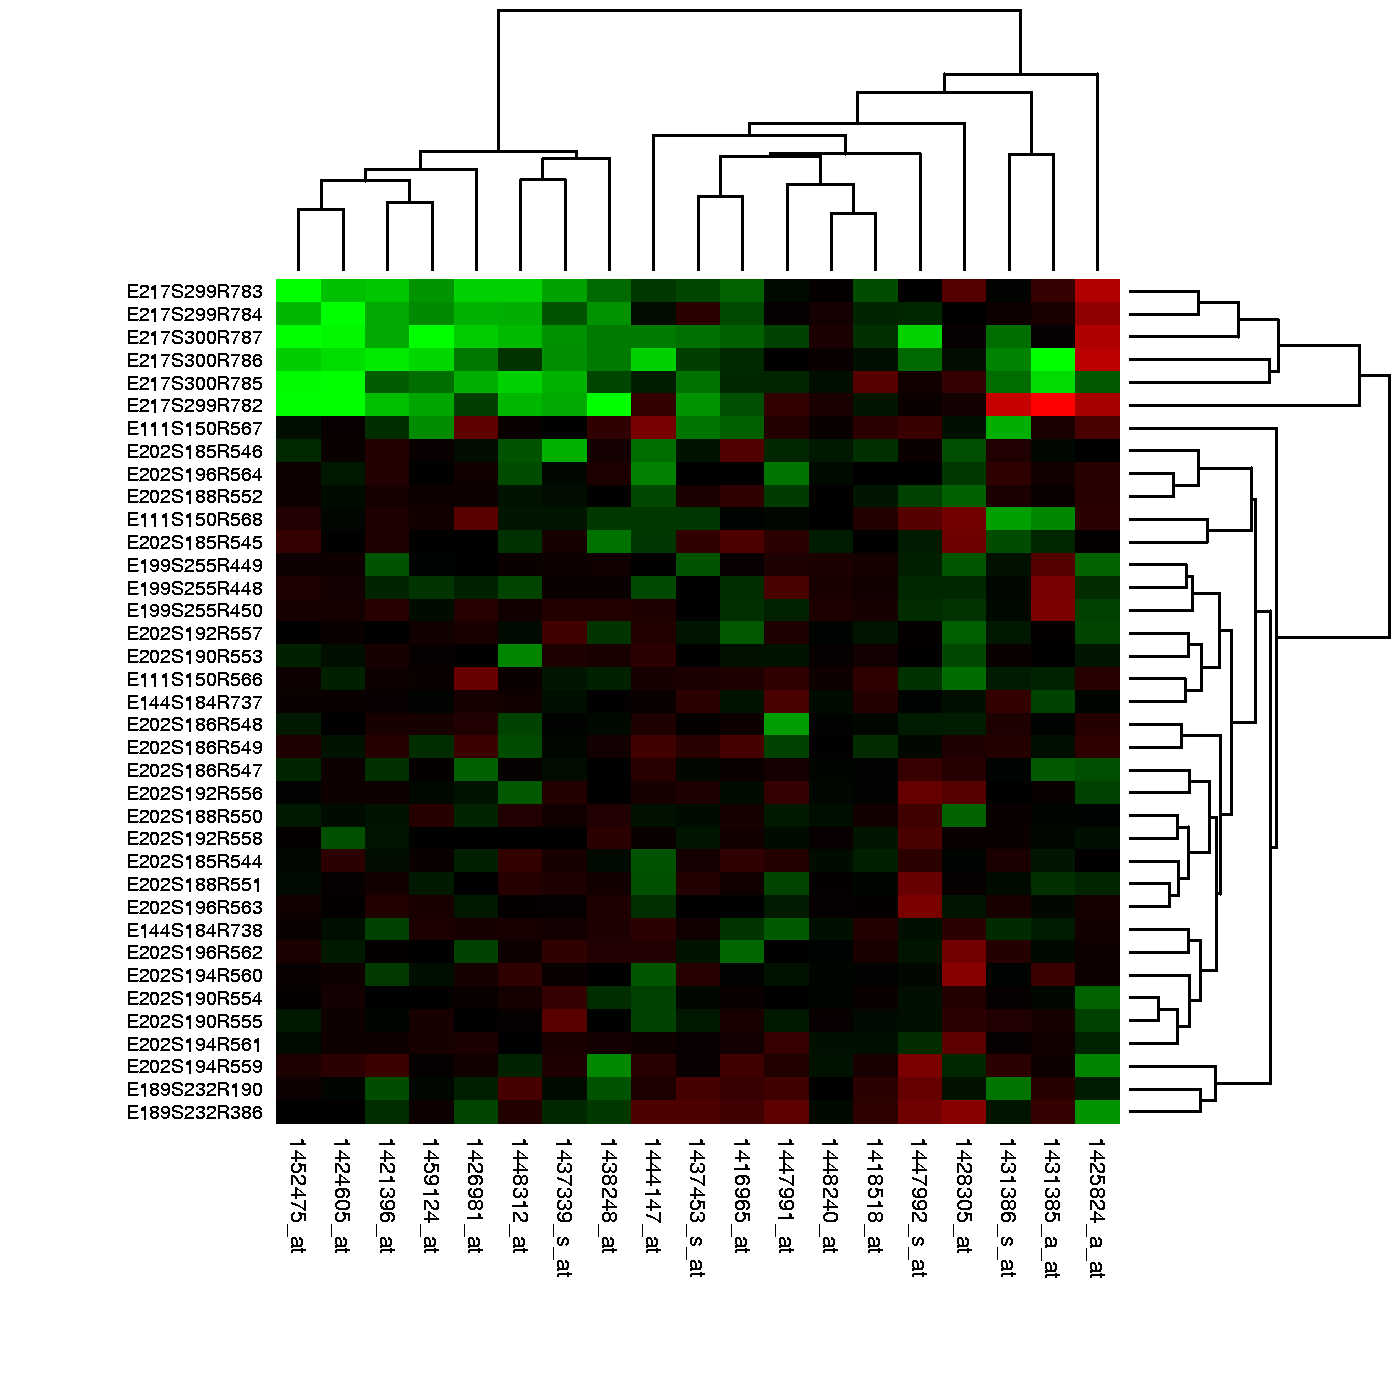
\includegraphics[width=2in]{L19-dnaarray.eps}
    \end{figure}


}    

\frame {
    \frametitle{\subsecname}
    \begin{itemize}
%    \center{Definition of Bi-clustering Problem}\\
    \item Input: a $n \times m$ matrix $A$.
    \item Output: a sub-matrix $A_{P,Q}$ of $A$ such that the rows of $A_{P,Q}$  are {\it similar}.
    That is, all the rows are identical.

    Why sub-matrix?\\
    A subset of  {\it genes} are co-regulated and co-expressed under specific {\it conditions}.
    It is interesting to find the subsets of genes and conditions.
    
    \begin{figure}
          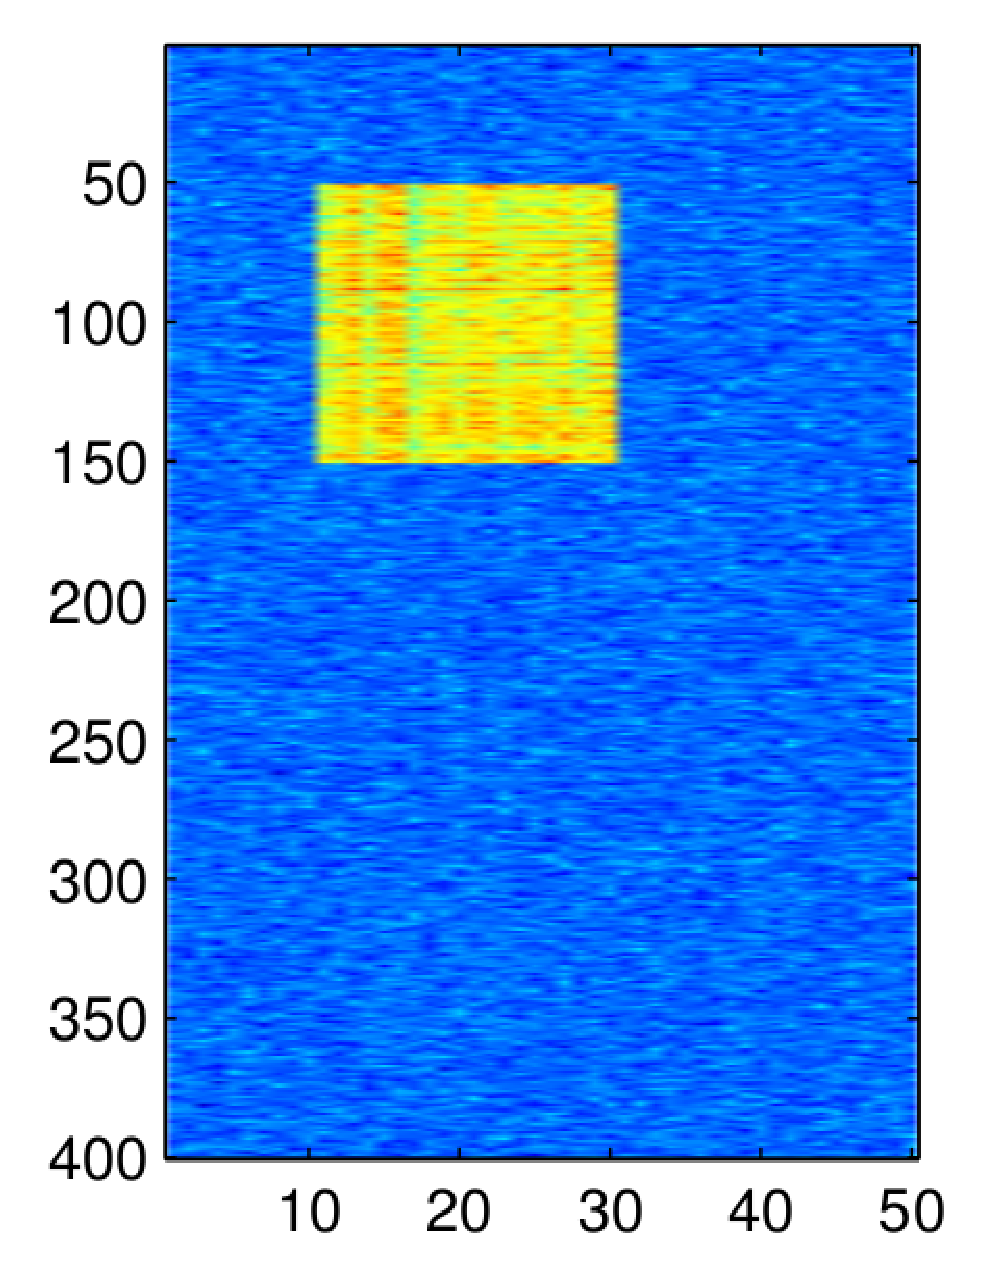
\includegraphics[width=2in]{L19-dnaarraybicluster.eps}
    \end{figure}
        
    \end{itemize}
    }

    \subsection{Similarity of Rows (1-5)}
    \frame {
    \frametitle{\subsecname}
    \begin{itemize}
    \item 1.  All rows are identical \\
       $1 ~1 ~2 ~3 ~2 ~3 ~3 ~2$ \\
       $1 ~1 ~2 ~3 ~2 ~3 ~3 ~2$ \\
       $1 ~1 ~2 ~3 ~2 ~3 ~3 ~2$ \\
    \item 2.  All the elements in a row are identical\\
       $1 ~1 ~1 ~1 ~1 ~1 ~1 ~1$\\
       $2 ~2 ~2 ~2 ~2 ~2 ~2 ~2$\\
       $5 ~5 ~5 ~5 ~5 ~5 ~5 ~5$\\
       (the same as 1 if we treat columns as
       rows)
    \end{itemize}
    }

    \frame {
    \frametitle{\subsecname}
    \begin{itemize}
    \item 3.  The curves for all rows are similar (additive)
       $a_{i,j}-a_{i,k} = c(j,k)$  for $i=1, 2, \ldots, m.$
       Case 3 is equivalent to case 2 (thus also case 1)  if we construct
       a new matrix $a^{*}_{i,j} =a_{i,j}-a_{i,p}$ for a fixed $p$ indicate a row.
       \begin{figure}
        \centering
        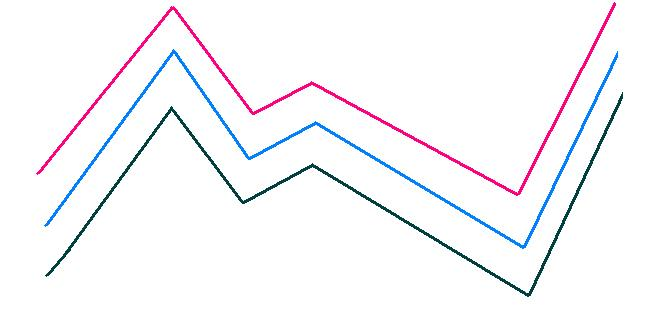
\includegraphics[scale=0.3]{curve.eps}
        \end{figure}
    \end{itemize}
    }

    \frame {
    \frametitle{\subsecname}
    \begin{itemize}
    \item 4. The curves for all rows are similar
    (multiplicative)\\
    $~~a_{1,1} ~~~~~ a_{1,2}~~~~~ a_{1,3}~~~~\ldots~~~~    a_{1,m}$ \\
    $c_{1}a_{1,1} ~~ c_{1}a_{1,2}~~ c_{1}a_{1,3} ~~~\ldots~~~
    c_{1}a_{1,m}$\\
    $c_{2}a_{1,1} ~~  c_{2}a_{1,2}~~  c_{2}a_{1,3} ~~~\ldots ~~~
    c_{2}a_{1,m}$\\
    $~~~\ldots ~~~$\\
    $c_{n}a_{1,1} ~~  c_{n}a_{1,2}~~  c_{n}a_{1,3} ~~~\ldots ~~~
    c_{n}a_{1,m}$
    \newline

    Transfer to case 2 (thus case 1) by taking log and
    subtraction.\\
    Case 3 and Case 4 are called bi-clusters with coherent values.
    \end{itemize}
    }

    \frame {
    \frametitle{\subsecname}
    \begin{itemize}
    \item 5.  The curves for all rows are similar
    (multiplicative and additive)
    \newline

    $a_{i,j}=c_{i}��a_{k,j} +d_{i}$
    \newline

    Transfer to case 2 (thus case 1) by subtraction of a fixed row
    (row i), taking log and subtraction of row i again.
    \newline
    The basic model: All the rows in the sub-matrix are identical.
    \end{itemize}
    }

    \subsection{Cheng and Church's model}
    \frame {
    \frametitle{\subsecname}
    The model introduced a similarity score called the mean squared residue score H  to measure the coherence of the rows and columns in the submatrix.
    \begin{eqnarray}
    H(P,Q)=\frac{1}{|P||Q|}\sum_{i\in P, j\in Q}(a_{i,j}-a_{i,Q}-a_{P,j}+a_{P,Q})^{2} \nonumber
    \end{eqnarray}
    where
    \begin{eqnarray}
    a_{i,Q}= \frac{1}{|Q|}\sum_{j\in Q}a_{i,j},~~ a_{P,j}=\frac{1}{|P|}\sum_{i\in P}a_{i,j}, a_{P,Q}=\frac{1}{|P||Q|} \sum_{i\in P, j\in Q}a_{i,j}. \nonumber
    \end{eqnarray}
    If there is no error, H(P, Q)=0 for case 1, 2 and 3. A lot of heuristics (programs) have been produced.
    }

    \frame{
    \frametitle{J. Liu's statistical model } 
\begin{figure}
          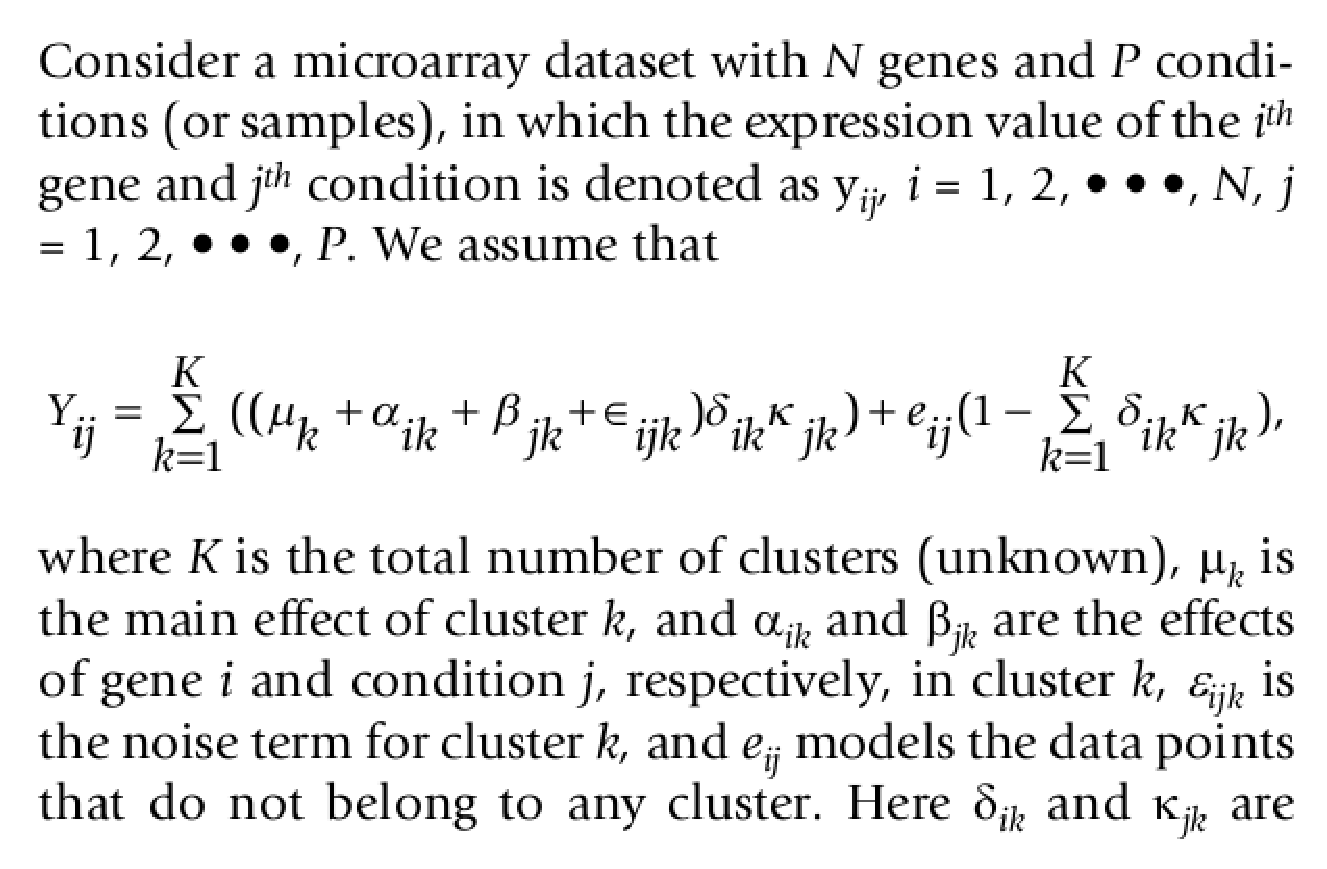
\includegraphics[width=4in]{L19-bayesianmodel.eps}
\end{figure}
    }


\section{Our Problem Definition}

    \subsection{Consensus Sub-matrix Problem}
    \frame {
    \frametitle{\subsecname}
    \begin{itemize}
    \item Input: a $n \times m$ matrix $A$, integers $l$ and $k$.
    \item Output: a sub-matrix $A_{P,Q}$ of $A$ with $l$ rows and $k$ columns and a consensus row $z$ (of $k$ elements)  such  that
    \newline

    $\sum_{r_{i}\in P}d(r_{i}|^{Q},z)$ is minimized.
    \newline

    Here $d(~,~)$ is the Hamming distance.
    \end{itemize}
    
    \begin{figure}
          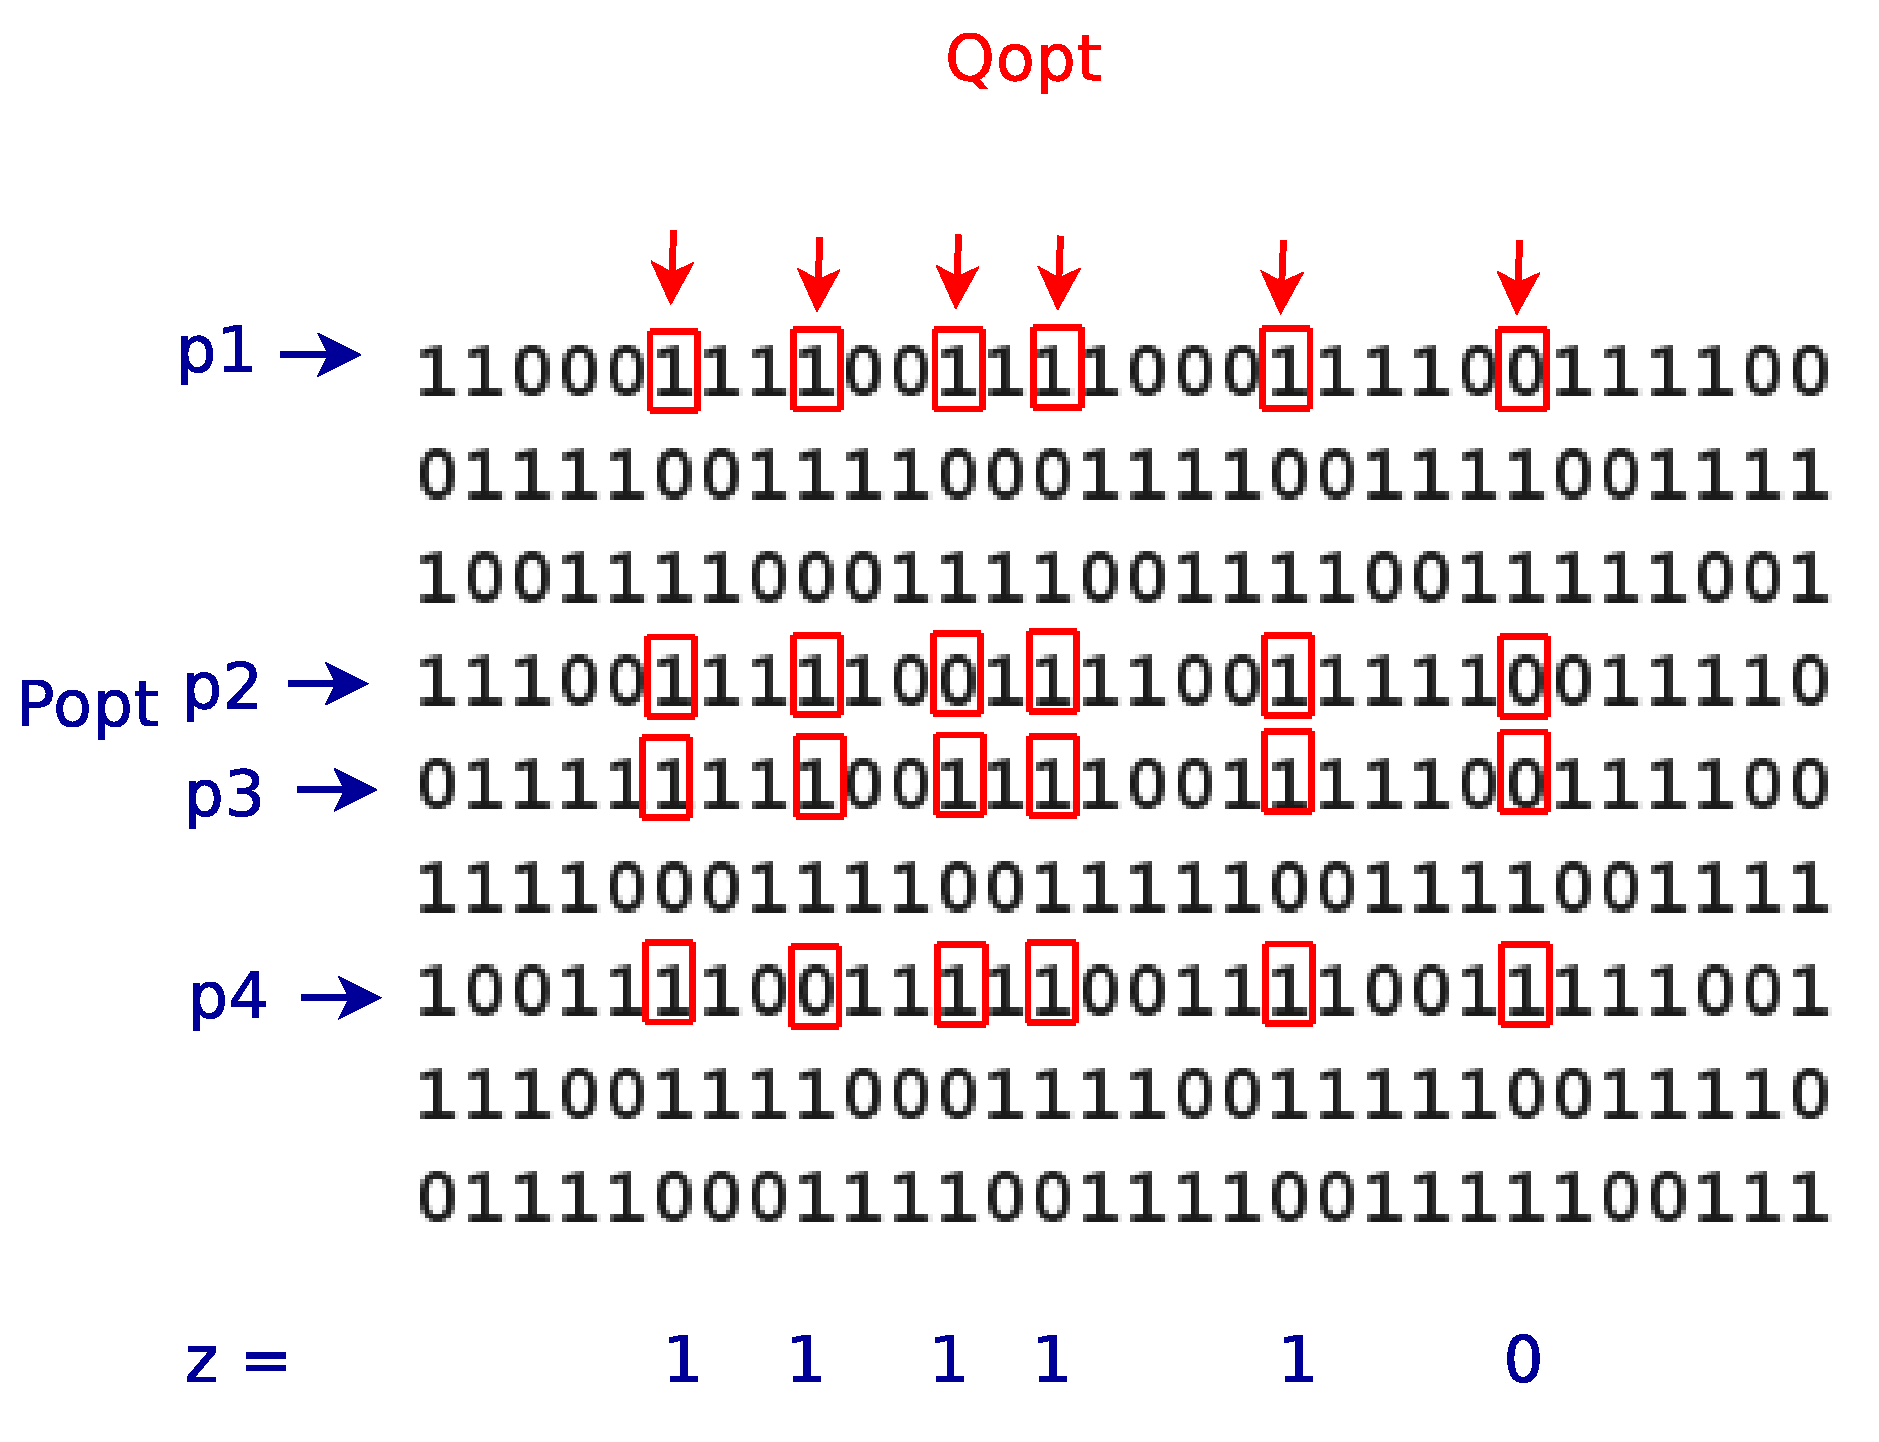
\includegraphics[width=2.5in]{L19-biclusteringexample.eps}
    \end{figure}
    }

    \subsection{Bottleneck  Sub-matrix Problem}
    \frame {
    \frametitle{\subsecname}
    \begin{itemize}
    \item Input: a $n \times m$ matrix $A$, integers $l$ and $k$.
    \item Output: a sub-matrix $A_{P,Q}$ of $A$ with $l$ rows and $k$ columns and a consensus row $z$ (of $k$ elements) such
    that for any $r_{i}$ in $P$
    \newline

    $d(r_{i}|^{Q},z) \leq d$ and $d$ is minimized
    \newline

    Here $d(~,~)$ is the Hamming distance.
    \end{itemize}
    }

    \subsection{NP-Hardness Results}
    \frame {
    \frametitle{\subsecname}
    \begin{itemize}
    \item Theorem 1: Both consensus sub-matrix and bottleneck sub-matrix problems are NP-hard.
    \newline

    Proof: We use a reduction from maximum edge bipartite problem.
    \end{itemize}
    }


\section{Approximation Algorithm for Consensus Sub-matrix Problem}

   \frame {
    \frametitle{\secname}
    \begin{itemize}
    \item Input: a $n \times m$ matrix $A$, integers $l$ and $k$.
    \item Output: a sub-matrix $A_{P,Q}$ of $A$ with $l$ rows and $k$ columns and a consensus row $z$ (of $k$ elements)  such   that
    \newline

    $\sum_{r_{i}\in P}d(r_{i}|^{Q},z)$ is minimized.
    \newline

    Here $d(~,~)$ is the Hamming distance.
    \end{itemize}
    }

    \subsection{Basic Ideas}
    \frame{
    \frametitle{Trial: brute-force}
      A brute-force method:
      \begin{itemize}
       \item By enumerating all size $k$ subset of columns, and all length $k$ vector, we could know $Q_{opt}$ and $z$ at some moment; 
       \item Then we can find $P_{opt}$ in poly-time to minimize the consensus score.
       \item However, the first step will take ${  n \choose k} \times 2^k$ time. 
       \end{itemize}
    }

    \frame {
    \frametitle{Our method}
	
    \begin{itemize}
       \item Basic idea: instead of the whole $Q_{opt}$ and $z_{opt}$, knowing a small part is enough. In other words, the whole $Q_{opt}$ can be approximated based on the small part. 
   \item Key questions: 
	\begin{enumerate}
	 \item What is the size of the small part? 
	 \item How to approximate the whole $Q_{opt}$ based on the small part? 
 	\item How to obtain such a small part? 
	\end{enumerate}

%     \item Assumptions: $H_{opt}=\sum_{p_{i}\in
%     P_{opt}}d(x_{p_{i}}|^{Q_{opt}},z_{opt})=O(kl)$, $H_{opt}
%     \times c' = kl$ and $|Q_{opt}|=k=O(n)$, $k \times c =n$.
%     \item Basic Ideas:  We use a random sampling technique to randomly select O(log$m$) columns in $Q_{opt}$,
%     enumerate all possible vectors of length O(log$m$) for those columns. At some moment, we know O(log$m$)
%     bits of $r_{opt}$ and we can use the partial $z_{opt}$ to select the $l$ rows which are closest to $z_{opt}$ in those O(log$m$) bits.
%     After that we can construct a consensus vector $r$ as follows: for each column, choose the (majority) letter that appears the most in each of the
%     $l$ letters in the $l$ selected rows. Then for each of the $n$ columns, we can calculate the number of mismatches between the majority letter
%     and the $l$ letters in the $l$ selected rows. By selecting the best
%     $k$ columns, we can get a good solution.
%     }
    \end{itemize}
    }

    \frame[allowframebreaks]{
    \textbf{ Algorithm 1 for The Consensus Submatrix Problem }\\
	Basic Ideas:  
	\begin{itemize}
	 \item 
We use a random sampling technique to randomly select O(log$m$) columns in $Q_{opt}$,
     enumerate all possible vectors of length O(log$m$) for those columns. 
	\item At some moment, we know O(log$m$)
     bits of $r_{opt}$ and we can use the partial $z_{opt}$ to select the $l$ rows which are closest to $z_{opt}$ in those O(log$m$) bits. 
	\item 
     After that we can construct a consensus vector $r$ as follows: for each column, choose the (majority) letter that appears the most in each of the
     $l$ letters in the $l$ selected rows. 
	\item Then for each of the $n$ columns, we can calculate the number of mismatches between the majority letter    and the $l$ letters in the $l$ selected rows. By selecting the best
     $k$ columns, we can get a good solution.
\end{itemize}
    \footnotesize{   \textbf{Input:}   one $m\times n$ matrix $A$, integers $l$ and $k$, and $\epsilon>
    0$\\
    \textbf{Output:}  a size $l$ subset $P$ of rows, a size $k$ subset $Q$ of columns and a length $k$ consensus vector
    $z$\\
    \textbf{Step 1:} randomly select a set $B$ of $\lceil(c+1)(\frac{4\log m}{\epsilon^{2}}+1)\rceil$ columns from
    $A$.\\
    (1.1) {\bf for}  every size $\lceil\frac{4\log m}{\epsilon^{2}}\rceil$  subset $R$ of $B$ {\bf
    do}\\
    (1.2) {\bf for}  every $z|^{R} \in \Sigma^{|R|}$ {\bf
    do}\\
    (a) {Select the best $l$ rows $P =\{p_{1},...,p_{l}\}$ that minimize $d(z|^{R}, x_{i}|^{R})$.}\\
    (b)  {{\bf for}  each column $j$ {\bf do}\\
    Compute $f(j)=\sum_{i=1}^{l}d(s_{j},a_{p_{i},j})$, where $s_{j}$ is the  majority element of the $l$ rows in $P$ in column
    $j$. Select the best $k$ columns $Q=\{q_{1},...,q_{k}\}$ with minimum value $f(j)$ and let $z(Q)=s_{q_{1}}s_{q_{2}}\ldots
    s_{q_{k}}$.}\\
    (c) {Calculate $H=\sum_{i=1}^{l}d(x_{p_{i}}|^{Q},z)$  of this
    solution.}\\
    \textbf{Step 2:} Output $P$, $Q$ and $z$ with minimum $H$. }
    }

    \frame{
    \frametitle{}
     \begin{figure}
          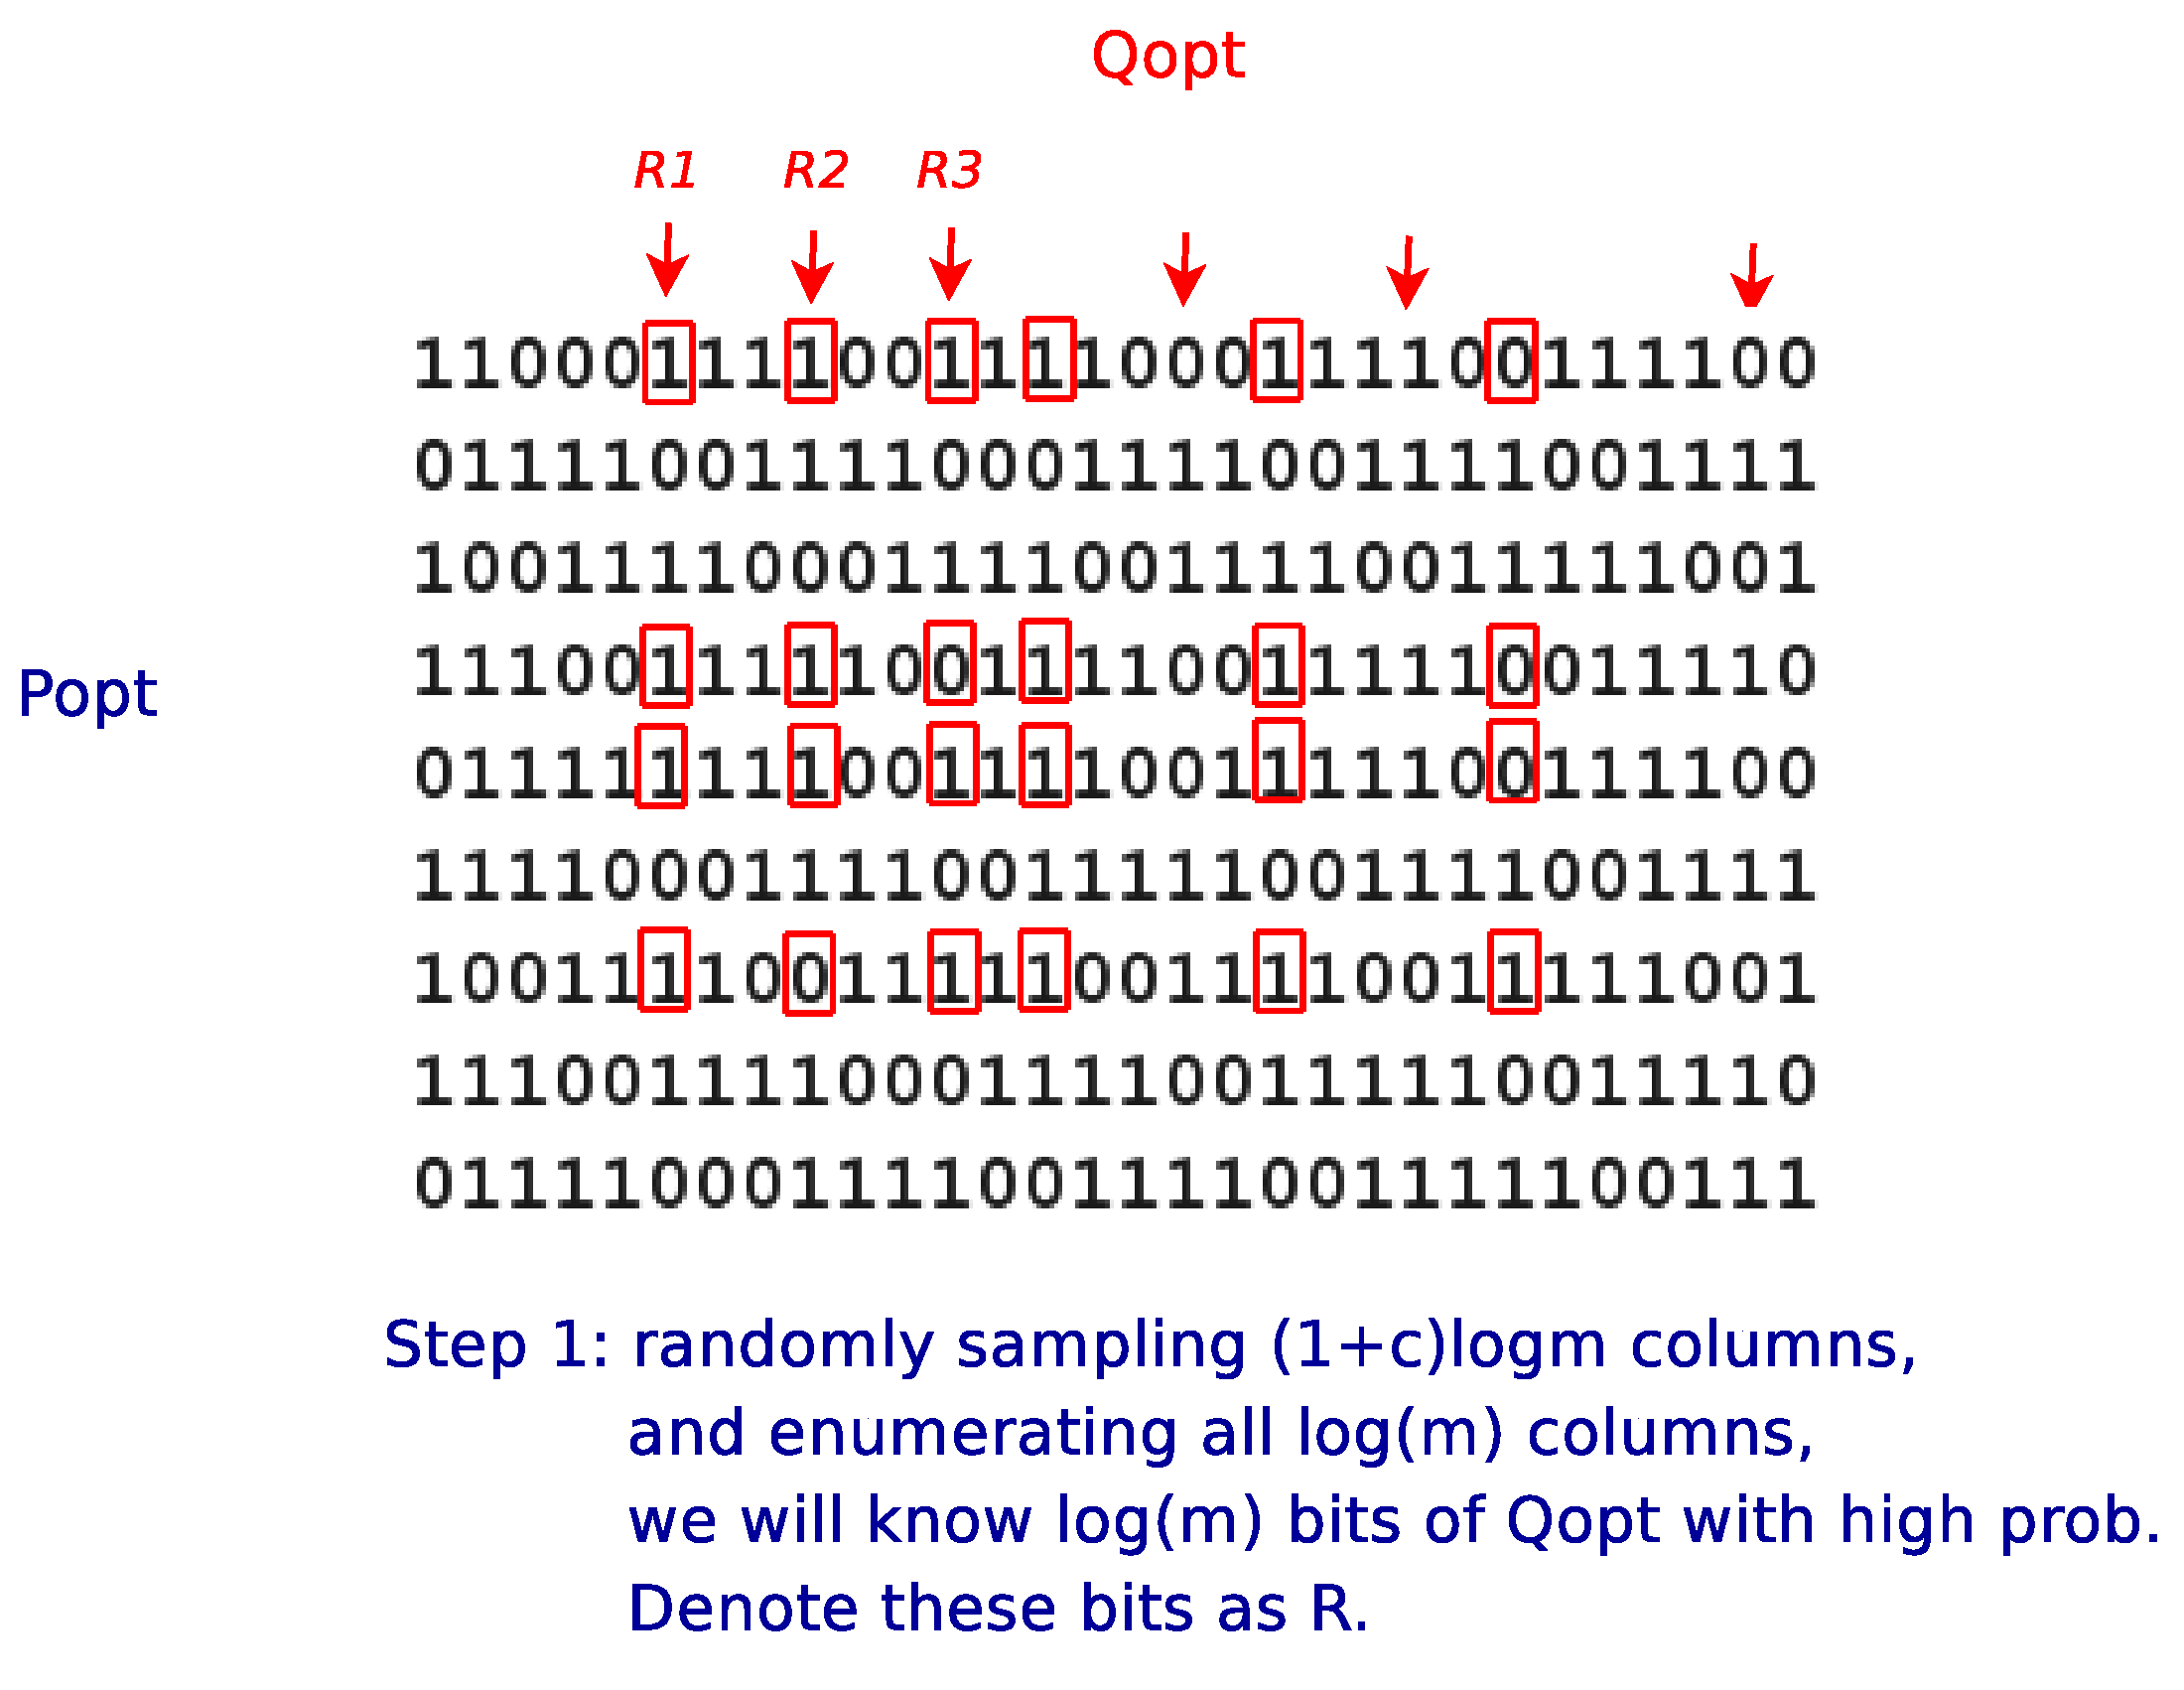
\includegraphics[width=4in]{L19-algo1step1.eps}
    \end{figure}
    } 
    \frame{
    \begin{figure}
          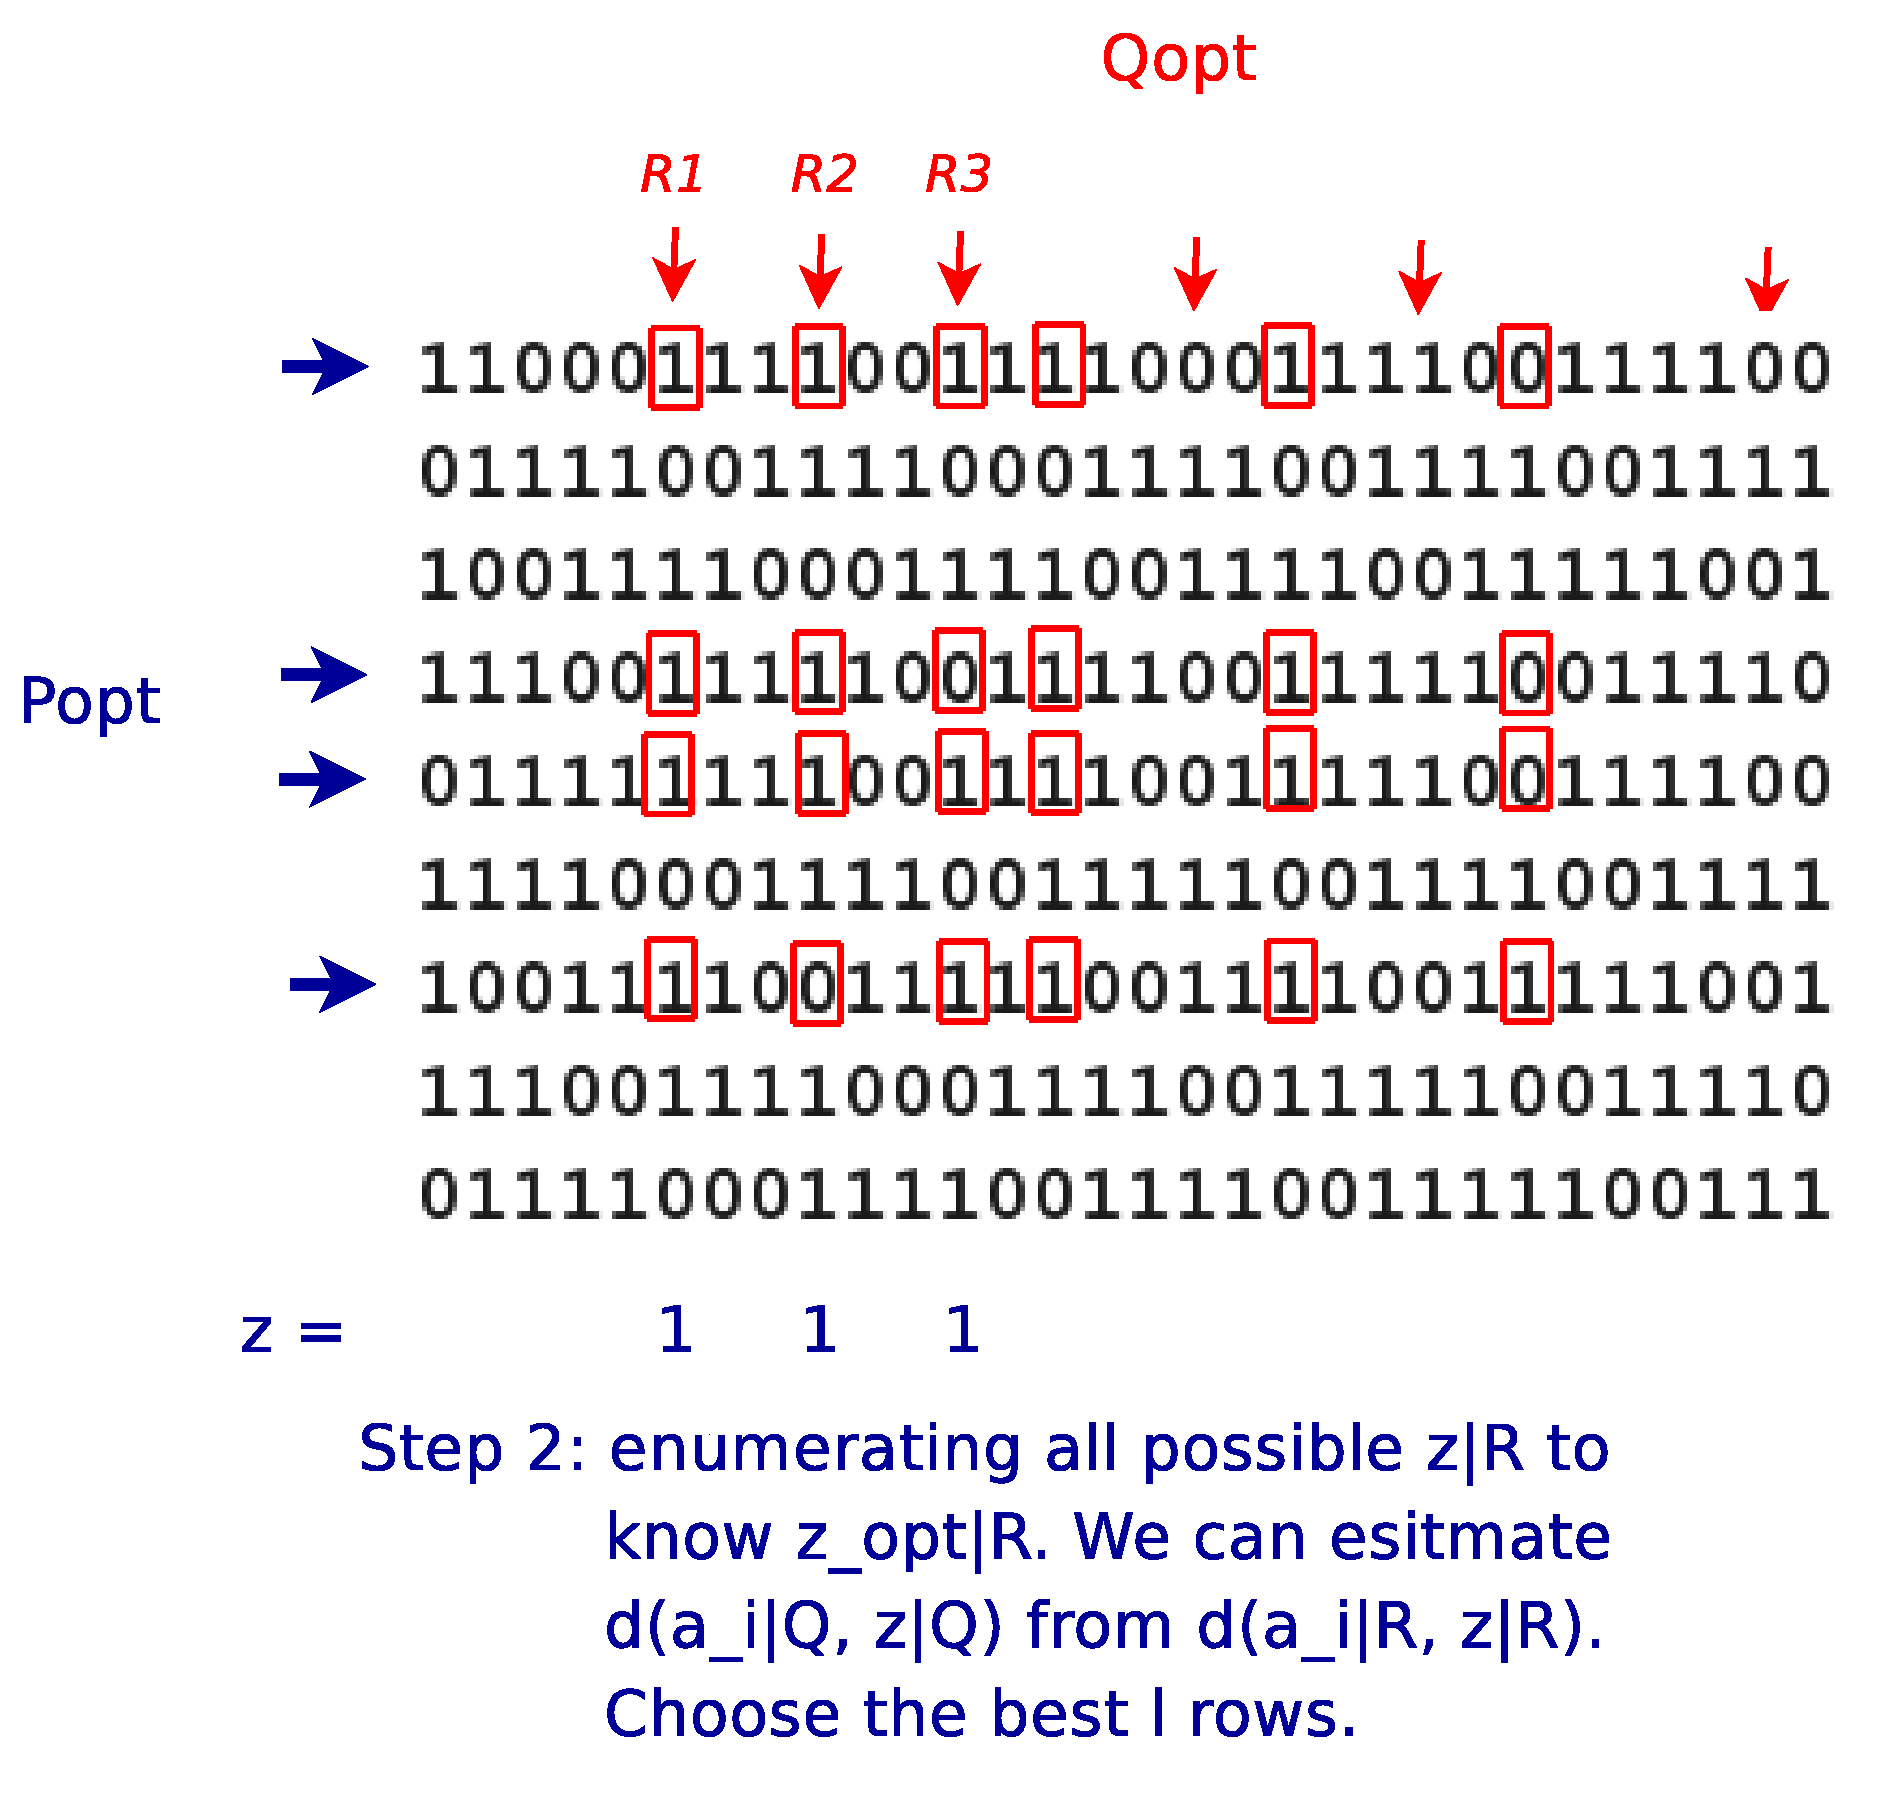
\includegraphics[width=3.5in]{L19-algo1step2.eps}
    \end{figure}
    } 
    \frame{
    \begin{figure}
          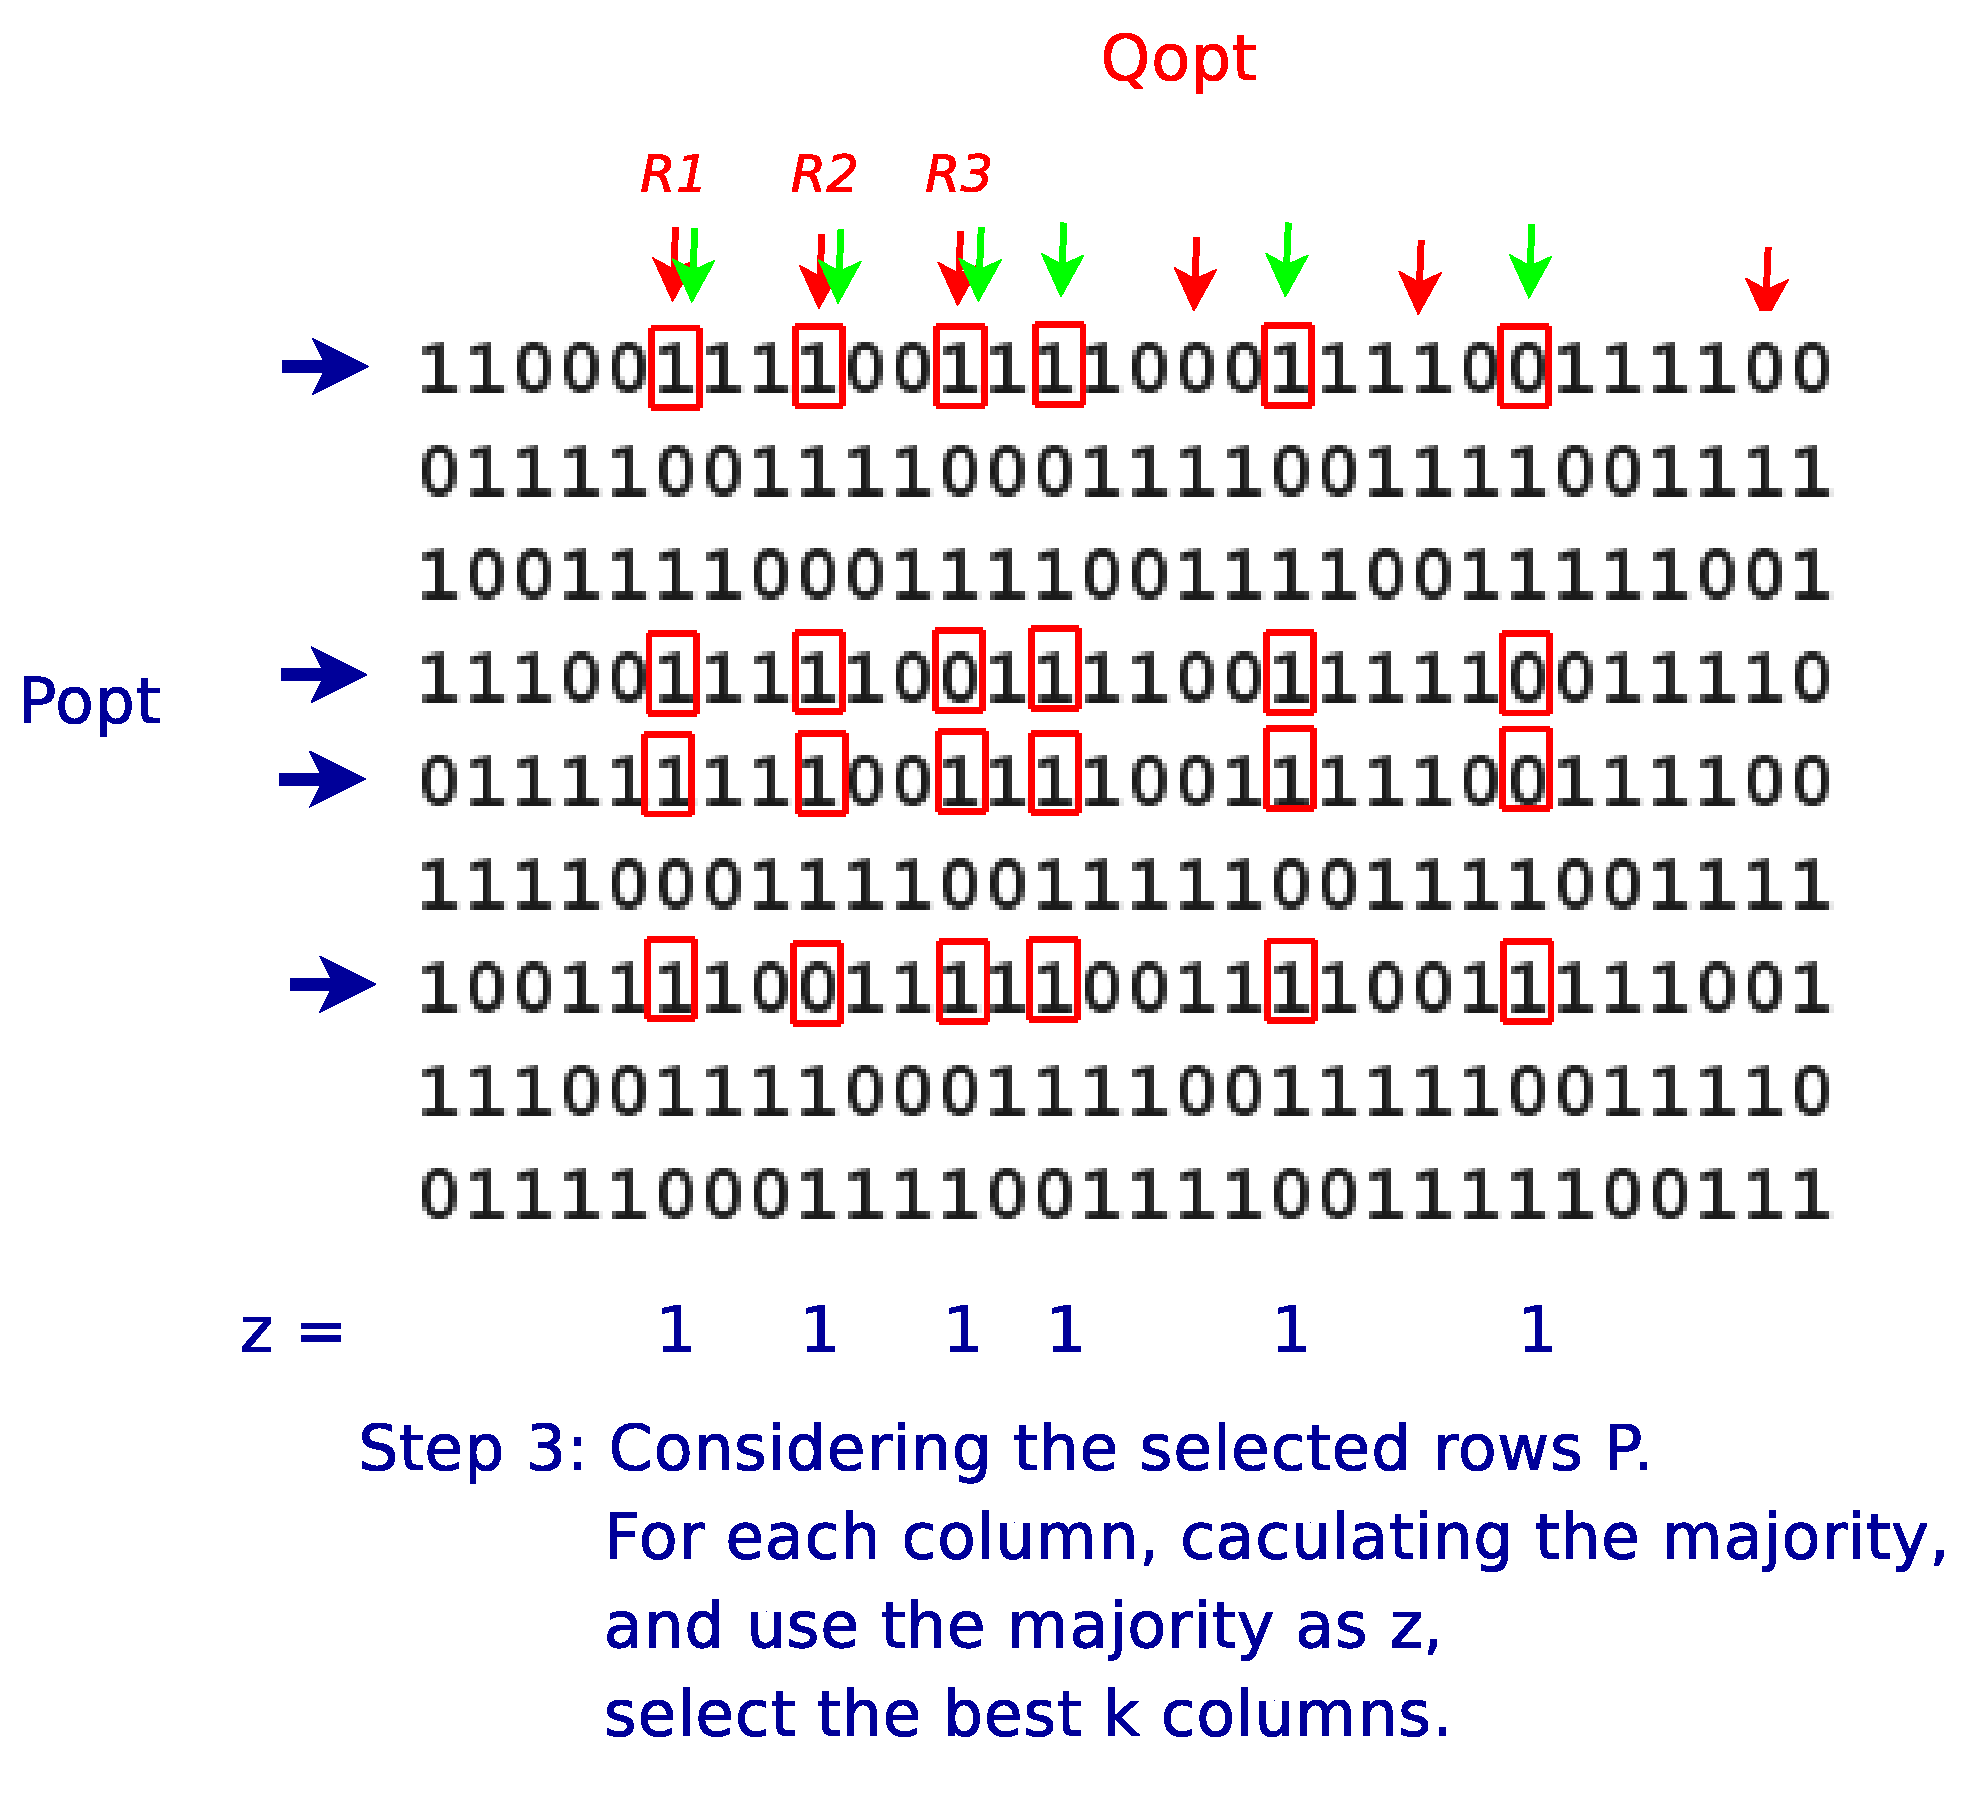
\includegraphics[width=3.5in]{L19-algo1step3.eps}
    \end{figure}
    }


    \frame[allowframebreaks]{
    \frametitle{Question 1,2: what size of ``small part'' is enough? how to approximate?}
Lemma 2: Randomly sample (with replaccement) of $R \subseteq Q_{opt}$, where $|R|=\lceil\frac{4\log m}{\epsilon^{2}}\rceil$ and. Let $\rho = \frac{k}{|R|}$. With probability at most $m^{-1}$, there is a row $a_{i}$ satisfying
        \begin{eqnarray}
        \frac{d(z_{opt}, a_{i}|^{Q_{opt}})-\epsilon k}{\rho}>d(z_{opt}|^{R}, a_{i}|^{R})
        .\nonumber
        \end{eqnarray}
        With probability at most  $m^{-\frac{1}{3}}$, there is a row $a_{i}$  satisfying
        \begin{eqnarray}
        d(z_{opt}|^{R}, a_{i}|^{R}) > \frac{d(z_{opt}, a_{i}|^{Q_{opt}})+\epsilon k}{\rho}
        .\nonumber
        \end{eqnarray}

Intuition: randomly sample a small subset of $Q_{opt}$ is enough!	

% \begin{figure}
%           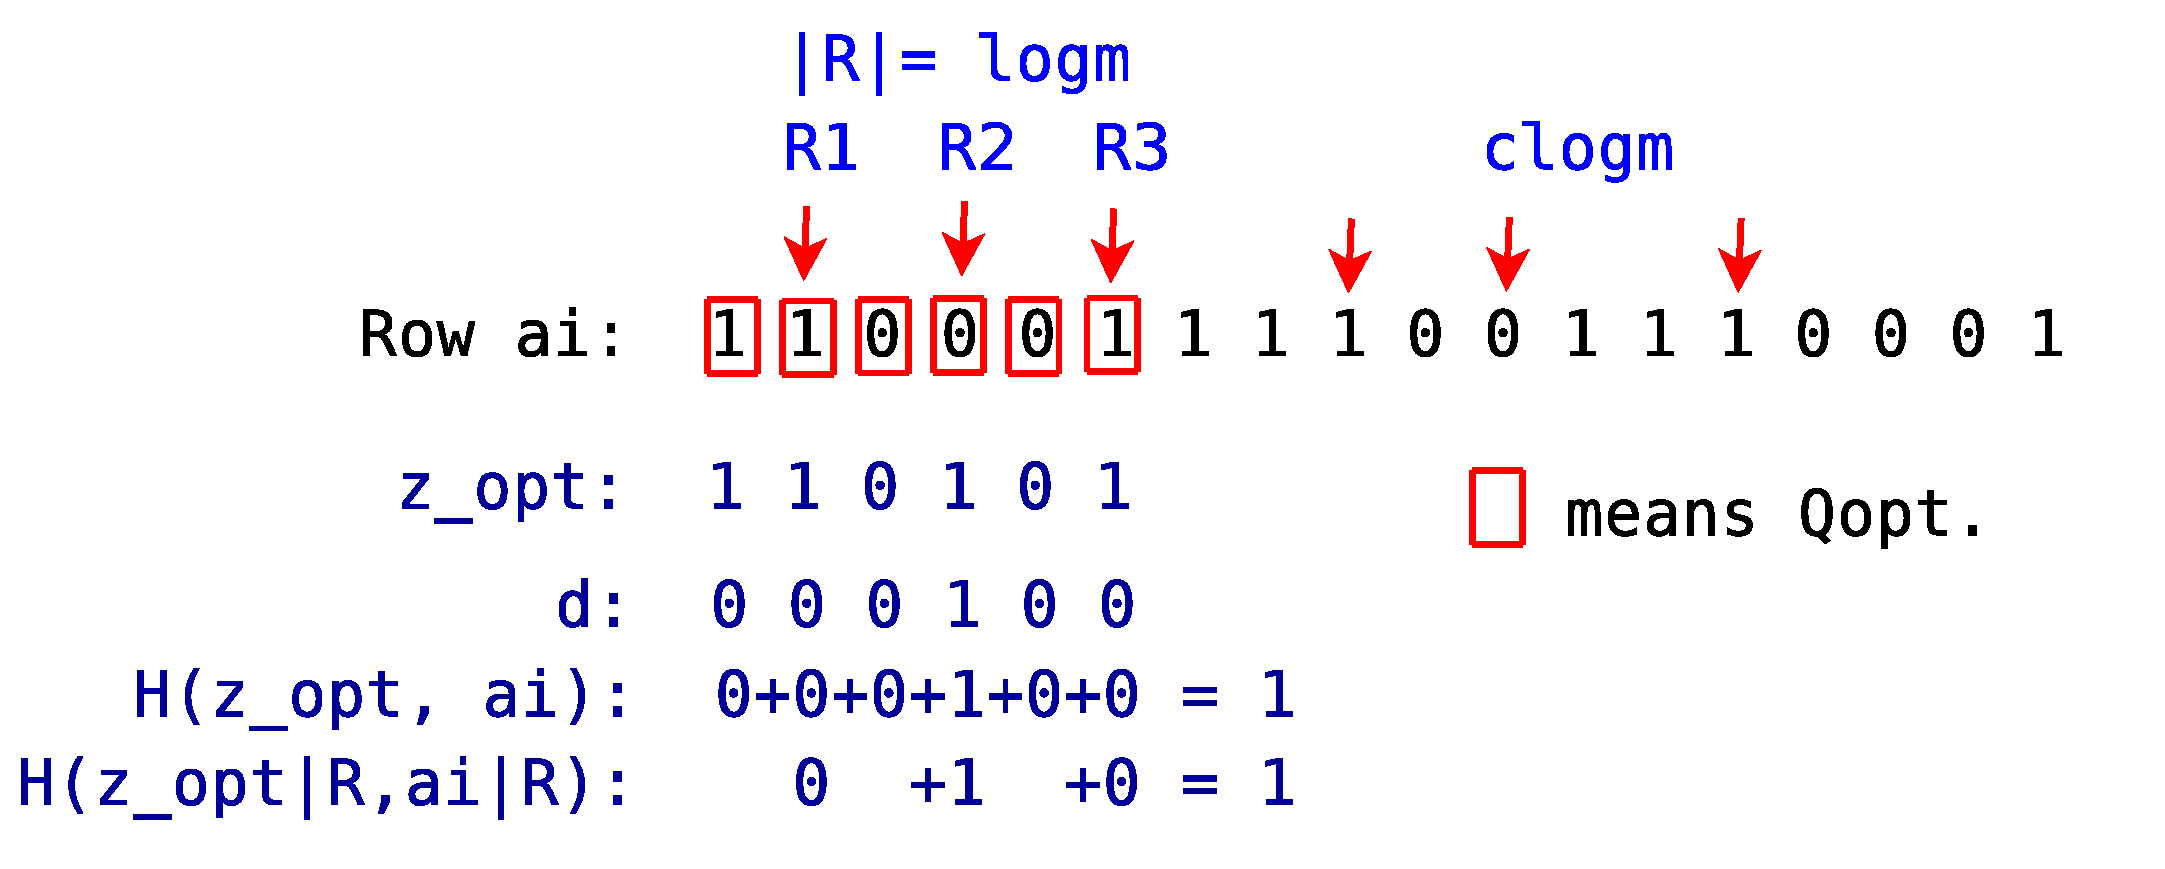
\includegraphics[width=3.5in]{L19-lemma3.eps}
% \end{figure}	
    }

    \frame[allowframebreaks]{
   % \frametitle{Question 1,2: what size of ``small part'' is enough? how to approximate?}
\begin{figure}
          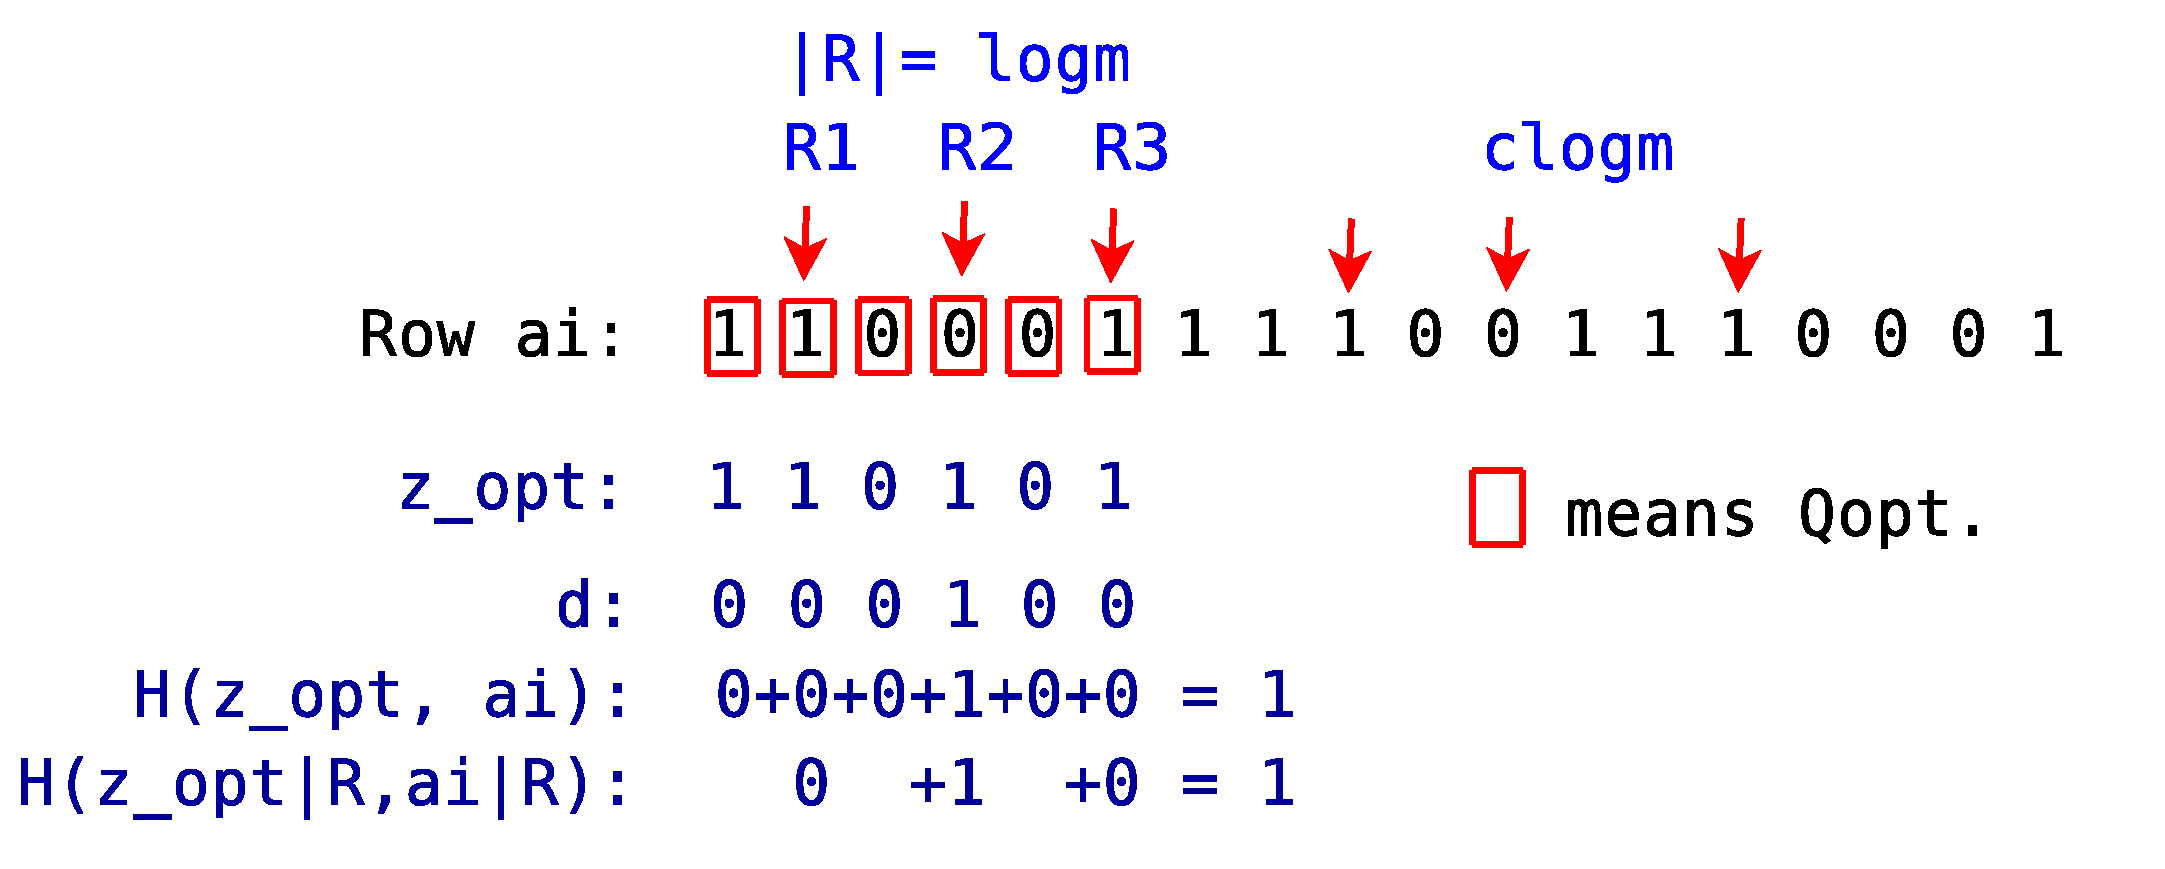
\includegraphics[width=3in]{L19-lemma3.eps}
\end{figure}	
	Proof: 
\begin{itemize}
 \item Define index variables $x_j=1$ if $j$ was selected into $R$, and $0$ otherwise. 
 \item $E( d(z_{opt}|^{R}, a_{i}|^{R}) )= \sum_{j=1}^k E(x_j) \times d_j = \frac{|R|}{k} d(z_{opt}, a_{i}|^{Q_{opt}})$.
 \item For any row $a_i$, \begin{eqnarray} 
&& \Pr( \frac{d(z_{opt}, a_{i}|^{Q_{opt}})-\epsilon k}{\rho}>d(z_{opt}|^{R}, a_{i}|^{R}) ) \nonumber \\
&\leq& exp( -\tfrac{1}{2} |R| \epsilon^2 )  \text{(by Chernoff bound)} \nonumber \\ 
&=& m^{-2}  \quad (\text{ set } |R|=\frac{4\log m}{\epsilon^{2}}) \nonumber 
\end{eqnarray}
\end{itemize}
 }


    \frame[allowframebreaks]{
    %\frametitle{Question 1,2: what size of ``small part'' is enough? how to approximate?}
    Lemma 3: When $R \subseteq Q_{opt}$ and $z|^{R}=z_{opt}|^{R}$, with probability at most $2 m^{-\frac{1}{3}}$,
    the set of rows $P=\{p_{1},\ldots,p_{l}\}$ selected in Step 1 (a) of Algorithm 1 satisfies $\sum_{i=1}^{l}d(z_{opt}, x_{p_{i}}|^{Q_{opt}}) > H_{opt} + 2\epsilon kl $. \\

   Intuition: $R$ can be used to approximate $Q_{opt}$.  \\

Proof: 
\begin{itemize}

\item With probability at most $m^{-1}$, $\sum_{i=1}{l} d(z_{opt}, a_i | Q_{opt} ) - \epsilon k l \geq \rho  \sum_{i=1}{l} d(z_{opt}|R, a_i | R ) $.
\item With probability at most $m^{-\tfrac{1}{3}}$, 
\begin{eqnarray}
H_{opt} & = & \sum_{i=1}{l} d(z_{opt}, a_i | Q_{opt} ) \nonumber \\ 
 &\leq & \rho  \sum_{i=1}{l} d(z_{opt}|R, a_i | R ) - \epsilon k l \nonumber 
\end{eqnarray}
\item Thus the lemma follows by the two facts.
\end{itemize}
}
	
    \frame[allowframebreaks] {
    \frametitle{ Question 3: how to obtain such a ``small part''? } 
    \begin{itemize}
   \item  Difficulty: How to randomly select O(log$m$) columns in $Q_{opt}$ while $Q_{opt}$ is unknown?

   \item Our idea: to randomly select a LARGER subset $B$ of $(c+1)$log$m$ columns, and enumerate all size log$m$ subsets of $B$ in poly-time  $O(m^{c+1})$. 
        

        \item  Lemma 1: With probability at most $m^{-\frac{2}{\epsilon^{2}c^{2}(c+1)}}$, no subset $R$ of size $\lceil\frac{4\log m}{\epsilon^{2}}\rceil$ used in Step 1 of Algorithm 1 satisfies  $R \subseteq
        Q_{opt}$.\\
 	\item Intuition: With high probability, we can get a set of log$m$ columns randomly selected from $Q_{opt}$.
        \end{itemize}

    \begin{figure}
          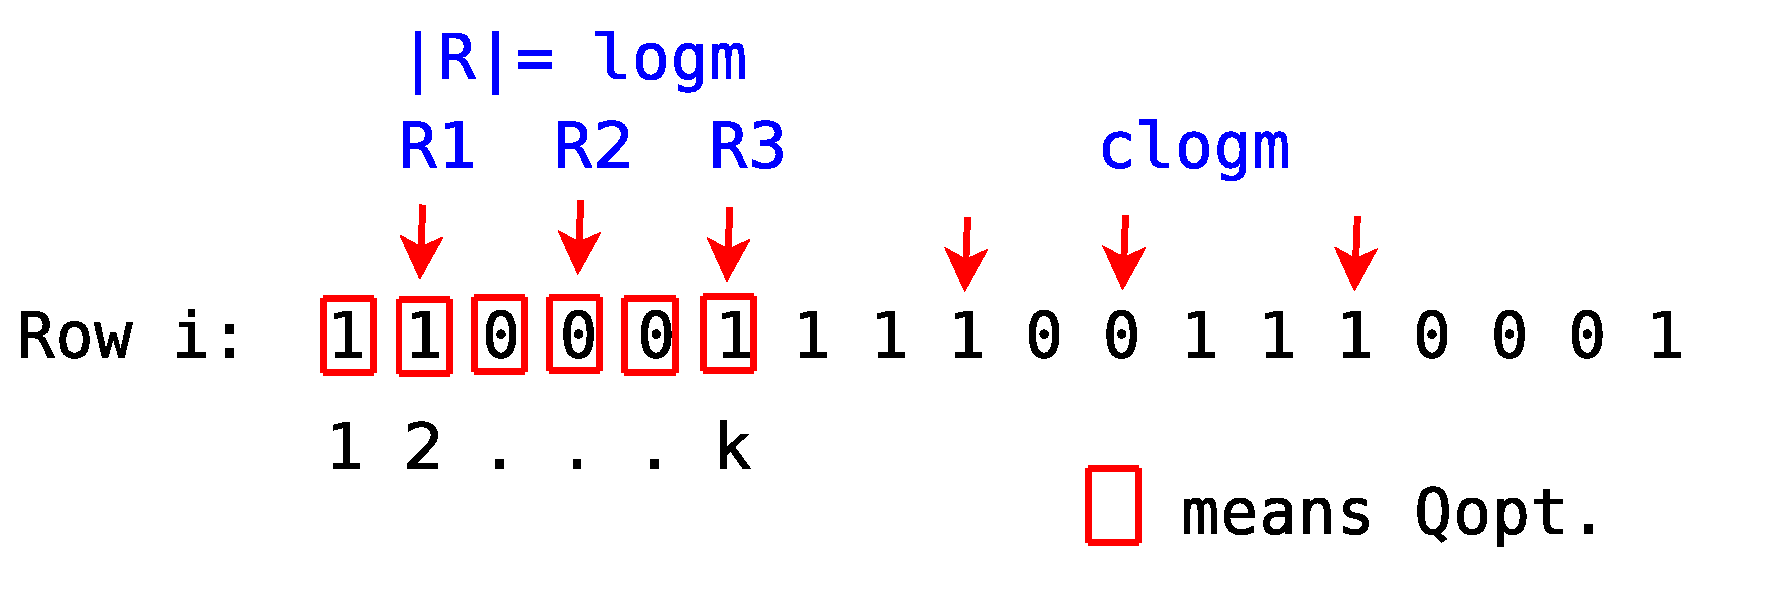
\includegraphics[width=2.5in]{L19-lemma2.eps}
    \end{figure}
Proof: 
\begin{itemize}
 \item Define index variables $x_j=1$ if the $j$-th trial hits a column in $Q_{opt}$, and $0$ otherwise.  Define $X=x_1+x_2+...+x_t$, where $t=(c+1)( \tfrac{4 \log m} {\epsilon^2} + 1 )$. 
 \item $E( X ) =  t \times k / n = c t   $  (assume $k=\Omega(n) = \tfrac{n}{c}$.)
 \item $\Pr( X \leq \tfrac{4log(m)}{\epsilon^2} )  \leq exp( -\tfrac{1}{2} t \epsilon^2 )$. 
\end{itemize}
 }

    \frame[allowframebreaks]{
    \frametitle{Analysis}
    \begin{itemize}
    \item Theorem 2: For any $\delta >0$, with probability at least $1-m^{-\frac{8c'^{2}}{\delta^{2}c^{2}(c+1)}}-2 m^{-\frac{1}{3}}$,
    Algorithm 1 will output a solution with consensus score at most $(1+ \delta)H_{opt}$ in  $O(nm^{O(\frac{1}{\delta^{2}})})$ time.
    
    \item Time-complexity: 
 \begin{enumerate}
    \item Step 1.1 is repeated $O( 2^{\tfrac{4(c+1)\log m}{\epsilon^2} } ) = O(m^{O(\tfrac{1}{\epsilon^2})}) = O(m^{O(\tfrac{1}{\delta^2})})$.
     \item Step 1.2 is repeated $O( m^{ O(\tfrac{\log{|\Sigma|} }{\epsilon^2}) } ) = O(m^{O(\tfrac{1}{\delta^2})})$.
   \item Total time: $O(n m^{O(\tfrac{1}{\delta^2})})$.
  \end{enumerate}

\end{itemize}

    }


\section{Approximation Algorithm for Bottleneck Sub-matrix Problem}

   \frame {
    \frametitle{\secname}
    \begin{itemize}
    \item Input: a $n \times m$ matrix $A$, integers $l$ and $k$.
    \item Output: a sub-matrix $A_{P,Q}$ of $A$ with $l$ rows and $k$ columns and a consensus row $z$ (of $k$ elements) such
    that for any $r_{i}$ in $P$
    \newline

    $d(r_{i}|^{Q},z) \leq d$ and $d$ is minimized
    \newline

    Here $d(~,~)$ is the Hamming distance.
    \end{itemize}
    }

    \subsection{Basic Ideas}
    \frame {
    \frametitle{\subsecname}
    \begin{itemize}
    \item Assumptions: $d_{opt}=MAX_{p_{i}\in P_{opt}}d(x_{p_{i}}|^{Q_{opt}},z_{opt})=O(k)$, $d_{opt} \times c''= k$ and $|Q_{opt}|=k=O(n)$, $k \times c =n$.
    \item Basic Ideas:\\
    (1) Use random sampling technique to know O(log$m$) bits of $z_{opt}$ and select $l$ best rows like Algorithm 1.\\
    (2) After knowing the $l$ rows, ``LP+RR'' technique is employed to select $k$ columns in the matrix.
    \end{itemize}
    }

   \frame {
    \begin{itemize}
    \item Linear programming\\
   \footnotesize{ Given a set of rows $P= \{ p_{1},\ldots,p_{l} \}$, we want to find a set of $k$ columns $Q$ and vector $z$ such that bottleneck score is
    minimized.\\
    \begin{eqnarray}
    && \min d; \nonumber \\
    && \sum_{i =1}^{n} \sum_{j=1}^{|\Sigma|}y_{i,j} = k, \nonumber \\
    && \sum_{j=1}^{|\Sigma|}y_{i,j} \leq 1, i = 1,2,\ldots,n, \nonumber \\
    && \sum_{i=1}^{n}\sum_{j=1}^{|\Sigma|}\chi(\pi_{j},x_{p_{s},i})y_{i,j}\leq d, s = 1,2,\ldots,l.\nonumber
    \end{eqnarray}
    }
    $y_{i,j}=1$ if and only if column $i$ is in $Q$ and the corresponding bit in $z$ is $\pi_{j}$.\\
    Here, for any $a,b \in \Sigma$, $\chi(a,b) = 0$ if $a = b$ and $\chi(a,b)=1$ if $a \neq b$.
    \end{itemize}
        }

   \frame {
    \begin{itemize}
    \item Randomized rounding\\
    To achieve two goals:\\
    (1) Select $k'$ columns, where $k'\geq k-\delta d_{opt}$.\\
    (2) Get integers values for $y_{i,j}$ such that the distance (restricted on the $k'$ selected columns) between any row in
    $P$
    and the center vector thus obtained is at most
    $(1+\gamma)d_{opt}$.\\
    Here $\delta>0$ and $\gamma>0$ are two parameters used to control the errors.
    \end{itemize}
    }

    \frame[allowframebreaks] {
    \begin{itemize}
    \item Lemma 4: When $\frac{n\gamma^{2}}{3(cc'')^{2}} \geq 2\log m$, for any $\gamma, \delta>0$, with probability at most
    $exp(-\frac{n\delta^{2}}{2(cc'')^{2}}) + m^{-1}$, the rounding result $y'=\{y'_{1,1},\ldots,y'_{1,|\Sigma|}, \ldots, y'_{n,1},\ldots,y'_{n,|\Sigma|}\}$ does not satisfy
    at least one of the following inequalities,
    \begin{eqnarray}
    \sum_{i=1}^{n}(\sum_{j=1}^{|\Sigma|}y'_{i,j}) > k - \delta
    d_{opt},\nonumber
    \end{eqnarray}
    and for every row $x_{p_{s}}(s = 1,2,\ldots,l)$,
    \begin{eqnarray}
    \sum_{i =1}^{n}
    (\sum_{j=1}^{|\Sigma|}\chi(\pi_{j},x_{p_{s},i})y'_{i,j}) <
    \overline{d} + \gamma d_{opt}.\nonumber
    \end{eqnarray}
    \item Intuition: random rounding can generate a good approximation, i.e., $k'\geq k-\delta d_{opt}$ columns along with an objective value $d \leq d_{opt} + r d_{opt}$
    \end{itemize}
    }
	
	\frame{
	\frametitle{ Proof}
	\begin{itemize}
	 \item Denote $Y=\sum_{i=1}^{n}(\sum_{j=1}^{|\Sigma|}y'_{i,j})$. We have $E(Y)=k$. 
	 \item \begin{eqnarray}
	        &&\Pr(Y \geq k - \delta d_{opt} ) \nonumber \\ 
		&\leq & exp( -\tfrac{1}{2} n (\tfrac{\delta d_{opt} }{ n }) ^2 )  \nonumber \\
		&\leq & exp( -\tfrac{1}{2} n (\tfrac{\delta  }{ c c'' }) ^2 ) 	\quad \text{( assume } d_{opt} = \Omega( k ) = \tfrac{k}{c''} = \tfrac{n}{c c''} ) \nonumber 
	       \end{eqnarray}
% 	\item \begin{eqnarray}
% 	        &&\Pr( Y \geq k - \delta d_{opt} ) \nonumber \\ 
% 		&\leq & exp( -\tfrac{1}{2} n (\tfrac{\delta d_{opt} }{ n }) ^2 )  \nonumber \\
% 		&\leq & exp( -\tfrac{1}{2} n (\tfrac{\delta  }{ c c'' }) ^2 ) 	\quad \text{( assume } d_{opt} = \Omega( k ) = \tfrac{k}{c''} = \tfrac{n}{c c''} ) \nonumber 
% 	       \end{eqnarray}
	\end{itemize}

	}


    \subsection{Approximation Algorithm}
    \frame {
    \textbf{Algorithm 2 for The bottleneck Sub-matrix Problem}
    \footnotesize{
    \textbf{Input:}   one matrix $A \in \Sigma^{m \times n}$, integer $l$, $k$, a row $z \in \Sigma^{n}$ and  small numbers $\epsilon > 0$, $\gamma>0$ and $\delta
    >0$.\\
    \textbf{Output:}  a size $l$ subset $P$ of rows, a size $k$ subset $Q$ of columns and a length $k$ consensus vector
    $z$.\\
    \textbf{if} $\frac{n\gamma^{2}}{3(cc'')^{2}} \leq  2\log m$ {\bf then} {try  all size $k$ subset $Q$ of the $n$ columns and all $z$ of length $k$ to solve the
    problem.}\\
    \textbf{if} $\frac{n\gamma^{2}}{3(cc'')^{2}} > 2\log m$ {\bf
    then}\\
    \textbf{Step 1:} randomly select a set $B$ of $\lceil\frac{4(c+1)\log m}{\epsilon^{2}}\rceil$ columns from $A$.
    {\bf for} every $\lceil\frac{4\log m}{\epsilon^{2}}\rceil$ size subset $R$ of $B$ {\bf
    do}\\
    {\bf for} every $z|^{R} \in \Sigma^{|R|}$ {\bf do}\\
    (a) Select the best $l$ rows $P =\{p_{1},...,p_{l}\}$ that minimize $d(z|^{R},
    x_{i}|^{R})$.\\
    (b)Solve the optimization problem by linear programming and randomized rounding to get $Q$ and
    $z$.\\
    \textbf{Step 2:} Output $P$,$Q$ and $z$ with minimum bottleneck score $d$.
    }
    }

    \subsection{Proofs}
    \frame {
    \frametitle{\subsecname}
    \begin{itemize}
    \item Lemma 5: When $R\subseteq Q_{opt}$ and $z|^{R}=z_{opt}|^{R}$, with probability at most  $2m^{-\frac{1}{3}}$, the  set of rows
    $P=\{p_{1},\ldots,p_{l}\}$ obtained in Step 1(a) of  Algorithm 2 satisfies $d(z_{opt}, x_{p_{i}}|^{Q_{opt}})> d_{opt} + 2\epsilon k $ for some row $x_{p_{i}}(1\leq i \leq l)$.
    \item Theorem 3: With probability at least $1-m^{-\frac{2}{\epsilon^{2}c^{2}(c+1)}}-2m^{-\frac{1}{3}}- exp(-\frac{n\delta^{2}}{2(cc'')^{2}}) -m^{-1}$, Algorithm 2 runs in time
    $O(n^{O(1)}m^{O(\frac{1}{\epsilon^{2}}+\frac{1}{\gamma^{2}})})$ and obtains a solution with bottleneck score at most $(1 + 2c''\epsilon+\gamma +\delta)d_{opt}$ for any fixed $\epsilon,~\gamma, ~\delta> 0$.
    \end{itemize}
    }

   \subsection{Thanks}
    \frame {
    \frametitle{\subsecname}
    \begin{itemize}
    \item Acknowledgements \\
    This work is fully supported by a grant from the Research Grants Council of the Hong Kong Special Administrative Region, China [Project No. CityU
    1070/02E].\\
    This work is collaborated with Dr. Lusheng Wang and Xiaowen
    Liu in City University of Hong Kong, Hong Kong, China.
    \end{itemize}
    }

    \frame{
    Let $X_1,X_2,\ldots,X_n$ be $n$ independent random 0-1 variables,
    where $X_i$ takes $1$ with probability $p_i$, $0<p_i<1$. Let
    $X=\sum _{i=1}^n X_i$, and $\mu=E[X]$. Then for any
    $0<\epsilon\leq 1$,
    \begin{eqnarray}
    {\bf Pr}(X>\mu+\epsilon\, n ) &<& e^{-\frac 13 n \epsilon ^2} ,\nonumber \\
    {\bf Pr}(X<\mu-\epsilon\,n ) &\leq& e^{ -\frac 12 n \epsilon ^2}.
    \nonumber
    \end{eqnarray}
    }



\end{document}
